%%% Endowing the Pisa/IIT SoftHand with the sense of touch

\subsubsection{Endowing the Pisa/IIT SoftHand with the sense of touch}
\label{sec:SenseOfTouch}

In~\ref{sec:imu2Fingers}, a modified version of the Mahony-Hamel passive complementary filter was used to obtain the orientation of a frame $\{ A \}$ with respect to another frame $\{ B \}$, expressed by a rotation matrix and subject to kinematic constraints, to reconstruct a two-finger gripper. In this section, we extend that work to the five-finger Pisa/IIT SoftHand and the potential application of object recognition without vision and using a naive recognizer to tackle problems devised in Task 3.2. The following sections describe the components of the proposed solution.

\paragraph{(a) The Madgwick Filter}

Sebastian Madgwick~\cite{MadgwickMARG} studied a new algorithm to tackle the singularities associated with the Euler parametrization by employing quaternions. The Madgwick filter is similar to the Mahony-Hamel filter in the use of a correction factor that depends on the data read from an IMU at each time step. Let be ${^b\omega_x}$, ${^b\omega_y}$ and ${^b\omega_z}$ angular rate measures (in $\rad s^{-1}$) with respect the IMU body frame $\{ B\}$ respectively about $x$, $y$ and $z$ axis and $^{b}\Omega$ a vector containing these measures as
\begin{equation}
\label{eq4_01}
^b \Omega = [ 0 \quad {^b\omega_x} \quad {^b\omega_y} \quad {^b\omega_z} ],
\end{equation}
the quaternion describing the rate of change of the earth frame $\{ A \}$ with respect to the sensor frame $\{ B \}$ can be written as
\begin{equation}
\label{eq4_02}
^b_a\dot{q} = \frac{1}{2} {^b_a \bar{q}}  \otimes {^b\Omega},
\end{equation}
where $\otimes$ denotes the quaternion product, and $\bar{}$ denotes the normalization operator. From~\eqref{eq4_02}, the orientation of the earth frame with respect to sensor frame at time \textit{t} is given by
\begin{equation}
\label{eq4_03}
^b_a \dot{q}_{\Omega,t} = \frac{1}{2} {^b_a \hat{\bar{q}}_{t-1}} \otimes ^b \Omega_t,
\end{equation}

\begin{equation}
\label{eq4_04}
^b_a q_{\Omega,t} = {^b_a \hat{\bar{q}}_{t-1}} + {^b_a \dot{q}_{\Omega,t}} \Delta t,
\end{equation}
where $^b \Omega_t$ is the angular rate measured at time \textit{t}, $\Delta t$ is the sampling period and $^b_a \hat{\bar{q}}_{t-1}$ is the previous estimate of the quaternion.

Now, by reading from a sensor a set of accelerometer and compass measurements in a frame strap down to the sensor, one can find infinite earth frame orientations.
%However, using quaternions, it is very easy to overcome the singularity problem, obtaining from sensors measures an unique orientation for the earth frame with respect the one attached to the sensor.
Thus, the orientation problem can be written as an optimization problem, where quaternion $^b_a \bar{q}$ aligns a predefined reference direction of a field (gravity or magnetic) in the earth frame $^a \bar{d}$ with the measured direction of the field in the sensor frame $^b \bar{s}$, stated as
\begin{equation}
\label{eq4_05}
\min_{{^b_a \bar{q}} \in \mathbb{R}^4} f({^b_a \bar{q}}, {^a \bar{d}}, {^b \bar{s}}),
\end{equation}
with the objective function defined as
\begin{equation}
\label{eq4_06}
f(^b_a \bar{q},^a \bar{d}, ^b \bar{s}) = ^b_a \bar{q}^{*} \otimes ^a \bar{d} \otimes ^b_a \bar{q} - ^b \bar{s},
\end{equation}
where $^b_a \bar{q}$ is the optimal quaternion, and $^a \bar{d} = [0 \quad d_x \quad d_y \quad d_z]$ and $^b \bar{s} = [0 \quad s_x \quad s_y \quad s_z]$ are the directions to be aligned in their respective reference frames. Here, $^{*}$ denotes the conjugate operator of a quaternion. 

The solution to~\eqref{eq4_05} can be found using a gradient descent strategy, which proved to be a satisfactory choice in terms of low computational burden and efficiency. Using an initial guess for the optimal quaternion~$^b_a \bar{q}_0$, it is possible to write the correction factor $^b_a \bar{q}_{k+1}$ linked to step $(k+1)$ as follows

\begin{equation}
\label{eq4_10}
^b_a q_{k+1} = ^b_a \bar{q}_k - \beta \frac{\nabla f(^b_a \bar{q}_k, ^a \bar{d}, ^b \bar{s})}{\vert \vert \nabla f(^b_a \bar{q}_k, ^a \bar{d}, ^b \bar{s}) \vert \vert}, \quad k = 0,1,2 \dots n,
\end{equation}
where
\begin{equation}
\label{eq4_10bis}
^b_a \bar{q}_k = \frac{1}{2} {^b_a \bar{q}_{k-1}} \otimes ^b{\Omega_k},  \quad k = 0,1,2 \dots n,
\end{equation}
\begin{equation}
\label{eq4_11}
\nabla f(^b_a \bar{q}_k, ^a \bar{d}, ^b \bar{s}) = J^T(^b_a \bar{q}_k,^a \bar{d}) f(^b_a \bar{q}_k, ^a \bar{d}, ^b \bar{s}),
\end{equation}
\begin{equation}
\label{eq4_12}
\begin{split}
f(^b_a \bar{q}_k, ^a \bar{d}, ^b \bar{s}) =
\left [ \begin{array}{c}
2d_x(\frac{1}{2} - q_3^2 - q_4^2) + 2d_y(q_1q_4 + q_2 q_3) + \\
2d_x(q_2 q_3 - q_1 q_4) + 2d_y(\frac{1}{2} - q_2^2 - q_4^2) + \\
2d_x(q_1 q_3 + q_2 q_4) + 2d_y(q_3 q_4 - q_1 q_2) + \end{array} \right. \\
\left. \begin{array}{r}
2 d_z(q_2q_4 - q_1q_3) - s_x \\
2d_z(q_1q_2 + q_3 q_4) - s_y \\
2d_z(\frac{1}{2} - q_2^2 - q_3^2) - s_z
\end{array} \right ] \end{split},
\end{equation}
\begin{equation}
\label{eq4_13}
\begin{split}
J(^b_a \bar{q}_k, ^a \bar{d}) =
\left [ \begin{array}{cc}
2d_yq_4 - 2d_zq_3 & 2d_yq_3+ 2d_zq_4\\
-2d_xq_4 + 2d_zq_2 & 2d_xq_3 - 4d_yq_2 + 2d_zq1 \\
2d_xq_3 - 2d_yq_2 & 2d_xq_4 - 2d_yq_1 - 4d_zq_2 \end{array} \right. \\
\left. \begin{array}{rr}
-4d_x q_3 2d_y q_2 - 2d_z q_1 & -4d_x q_4 2d_y q_1 + 2d_z q_2\\
2d_x q_2 + 2d_z q_4 &  -2d_x q_1 - 4d_y q_4 + 2d_z q_3\\
2d_x q_1 + 2 d_y q_4 - 4 d_z q_3 & 2 d_x q_2 + 2d_y q_3
\end{array} \right ] \end{split},
\end{equation}
with $\beta$ being the step size, and $J^T$ denoting the transpose of the Jacobian matrix of the objective function $f$.

Eq.~\eqref{eq4_05} defines a general alignment problem. Therefore, by considering measurements from accelerometers and magnetometers, it is possible to write two different problems: the first one using accelerometers data $f_g(^b_a \overline{q}_k, ^a \overline{g}_a, ^b \overline{g}_b)$ where $^a\overline{g}_a = \overline{g}_a$ is the gravity field measured in the inertial frame and $^b \overline{g}_b = \overline{g}_b$ is the gravity field in the sensor frame, and the second using the magnetometer data $f_m(^b_a \overline{q}_k, ^a \overline{m}_a, ^b \overline{m}_b)$ where $^a\overline{m}_a = \overline{m}_a$ is the magnetic field read in the inertial frame and $^s \overline{m}_b = \overline{m}_b$ is the magnetic field in the sensor frame. 

The two problems are combined to obtain a unique quaternion of the inertial frame with respect to the sensor frame as follows
\begin{equation}
\label{eq4_14}
f_{g,m}(^b_a \overline{q},\overline{g}_a,\overline{g}_b,\overline{m}_a,\overline{m}_b) = \left [ \begin{array}{c} f_g(^b_a \overline{q}, \overline{g}_a, \overline{g}_b) \\  f_m(^b_a \overline{q},  \overline{m}_a,  \overline{m}_b) \end{array} \right ].
\end{equation}
The expression of the optimal quaternion using again the gradient descent strategy at $(k+1)$ is
\begin{equation}
\label{eq4_15}
^b_a q_{k+1} = ^b_a \overline{q}_k - \beta \frac{\nabla f_{g,m}(^b_a \overline{q}_k,\overline{g}_a,\overline{g}_b,\overline{m}_a,\overline{m}_b) }{\vert \vert \nabla f_{g,m}(^b_a \overline{q}_k,\overline{g}_a,\overline{g}_b,\overline{m}_a,\overline{m}_b)  \vert \vert}, \quad k = 0,1,2 \dots n,
\end{equation}
where
\begin{equation}
\begin{split}
\label{eq4_16}
\nabla f_{g,m}(^b_a \overline{q}_k,\overline{g}_a,\overline{g}_b,\overline{m}_a,\overline{m}_b) = J_{g,m}^T(^b_a \overline{q}_k, \overline{g_a},\overline{m_a}) \\ {f}_{g,m}(^b_a \overline{q}_k,\overline{g}_a,\overline{g}_b,\overline{m}_a,\overline{m}_b),
\end{split}
\end{equation}
and
\begin{equation}
\label{eq4_17}
J_{g,m}^T(^b_a \overline{q}_k, \overline{g_a}, \overline{m_a}) = \left [ \begin{array}{c} J_g(^b_a \overline{q}_k,\overline{g}_a) \\ J_m(^b_a \overline{q}_k, \overline{m}_a) \end{array} \right ],
\end{equation}
with $J_g$ and $J_m$ the Jacobians of $f_g$ and $f_m$, respectively.

Fig.~\ref{BlockDiagram} shows the block diagram of the Madgwick filter. 
%Algorithm~\ref{MadgwickAlg} details the steps followed to obtain the orientation quaternion using its previous estimation and the data read from IMU, using $g_a$ and $m_a$ to denote, respectively, the gravity and the magnetic field in the inertial frame. 
In particular, the gravity field in the inertial frame is typically set as $g_a = [0 \quad 0 \quad 0 \quad 1]$, or rather, using a North-East-Down convention. The earth magnetic field in the inertial frame can be considered to have two components: one along the horizontal axis and one in the vertical axis, with its vertical component due to the inclination of the field depending on the latitude. In Pisa, for instance, it is about $1\degree$ w.r.t. the horizontal, so $m_a = [0 \quad m_{a_x} \quad 0 \quad m_{a_z}]$.

\begin{figure}[t]
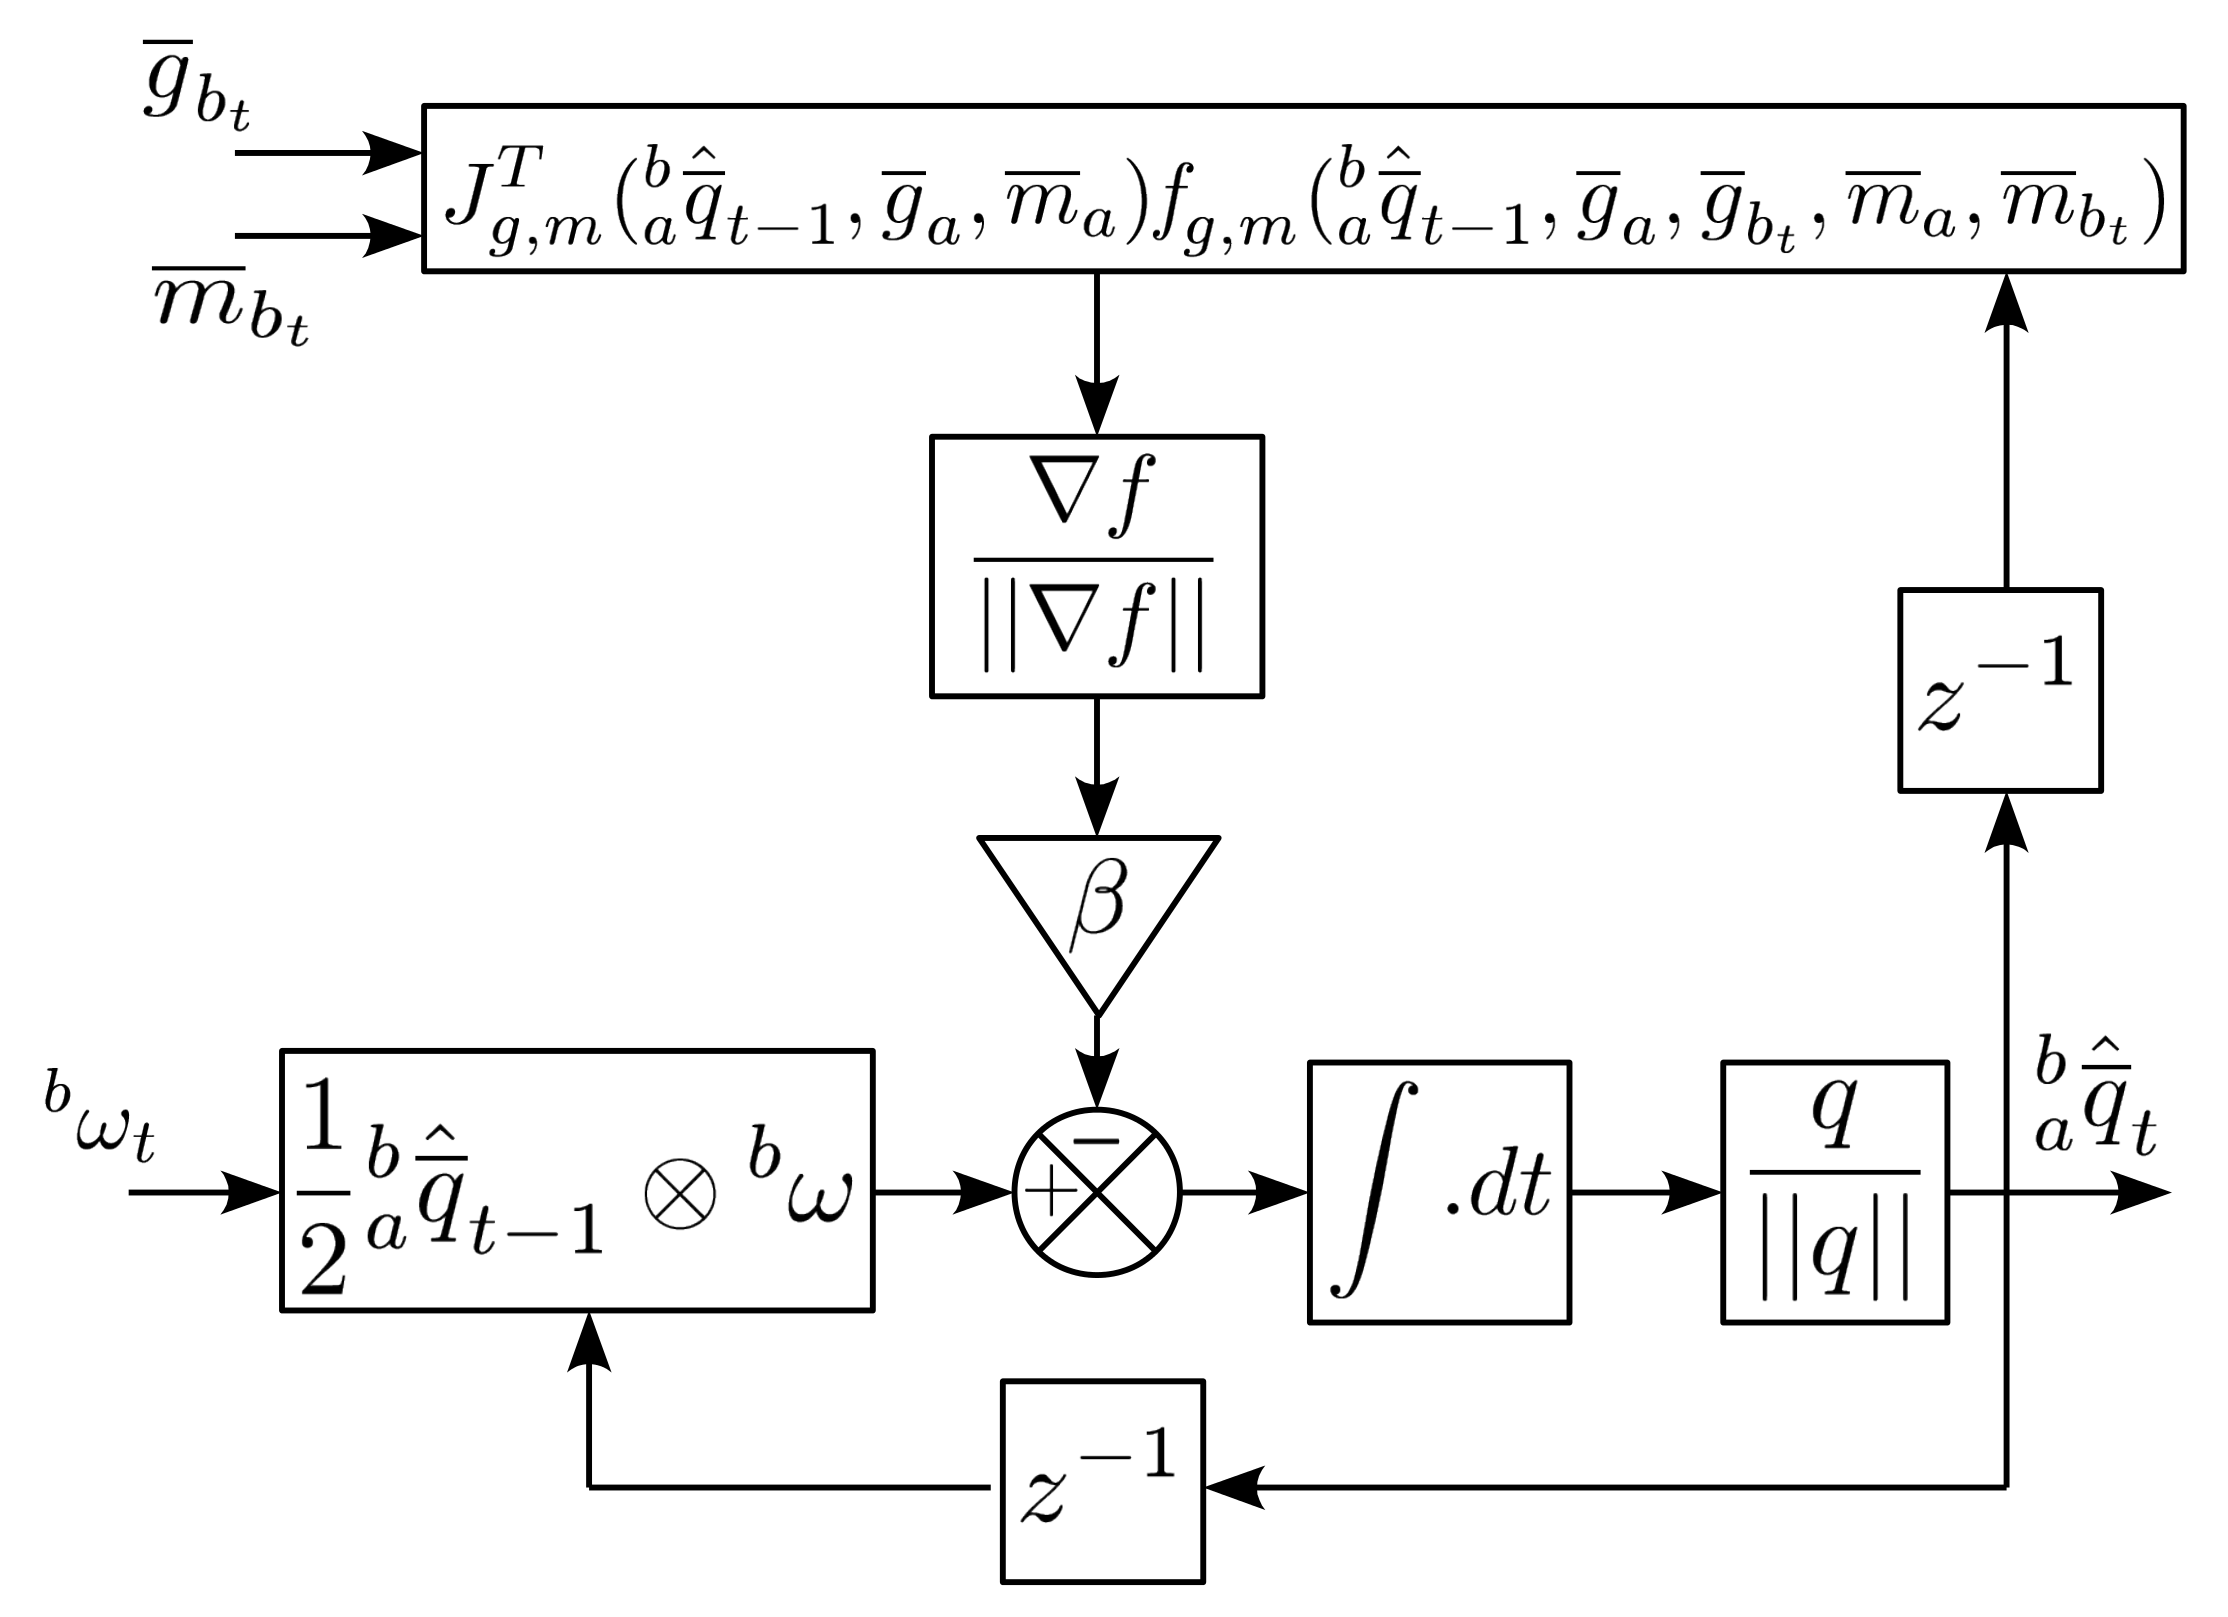
\includegraphics[scale=0.45]{Madgwick_Block_Diagram}
\caption{Block diagram of the Madgwick passive complementary filter}
\label{BlockDiagram}
\end{figure}

% \begin{algorithm}
% \caption{Madgwick Discrete Filter at $n^{th}$ step}
% \begin{algorithmic}[1]
% \label{MadgwickAlg}
% \STATE Reading the current values of the accelerometers ($g_{b_n}$), magnetometers ($m_{b_n}$) and gyro rates ($\Omega_{b_n}$) in the local IMU frame $\{B\}$
% \STATE Normalizing gravity and magnetic field vector read from IMU $\overline{g}_{b_n} = \frac{g_{b_n}}{\vert \vert g_{b_n} \vert \vert}$, $\overline{m}_{b_n} \frac{m_{b_n}}{\vert \vert m_{b_n} \vert \vert}$
% \STATE Computing the objective function value $f_{g,m}({^b_a\hat{\overline{q}}_{n-1}},\overline{g}_a,\overline{g}_{b_n},\overline{m}_a,\overline{m}_{b_n})$ using equations (\ref{eq4_12}) and (\ref{eq4_14})
% \STATE Computing the transpose of the Jacobian of the objective function $J^T_{g,m}(^b_a\hat{\overline{q}}_{n-1},\overline{g_a},\overline{m}_a)$ using equations (\ref{eq4_13}) and (\ref{eq4_17})
% \STATE Computing the correction terms $c_n =  \beta \frac{\nabla f}{\vert \vert \nabla f \vert \vert}$ using equation (\ref{eq4_16})
% \STATE Computing the orientation quaternion time variation $^b_a \hat{q}_{d_n} =  (\frac{1}{2} {^b_a\hat{\overline{q}}_{n-1}} \otimes \Omega_{b_n}) - c_n$
% \STATE Computing the new orientation quaternion estimation given by its previouly one and its current time variation $^b_a \hat{q}_n = ^b_a\hat{\overline{q}}_{n-1} + ^b_a \hat{q}_{d_n} \Delta t$
% \STATE Normalizing the new estimated quarternion $^b_a \hat{\overline{q}}_n = \frac{^b_a \hat{q}_n}{\vert \vert ^b_a \hat{q}_n \vert \vert}$
% \end{algorithmic}
% \end{algorithm}

\begin{figure}[t]
\centering
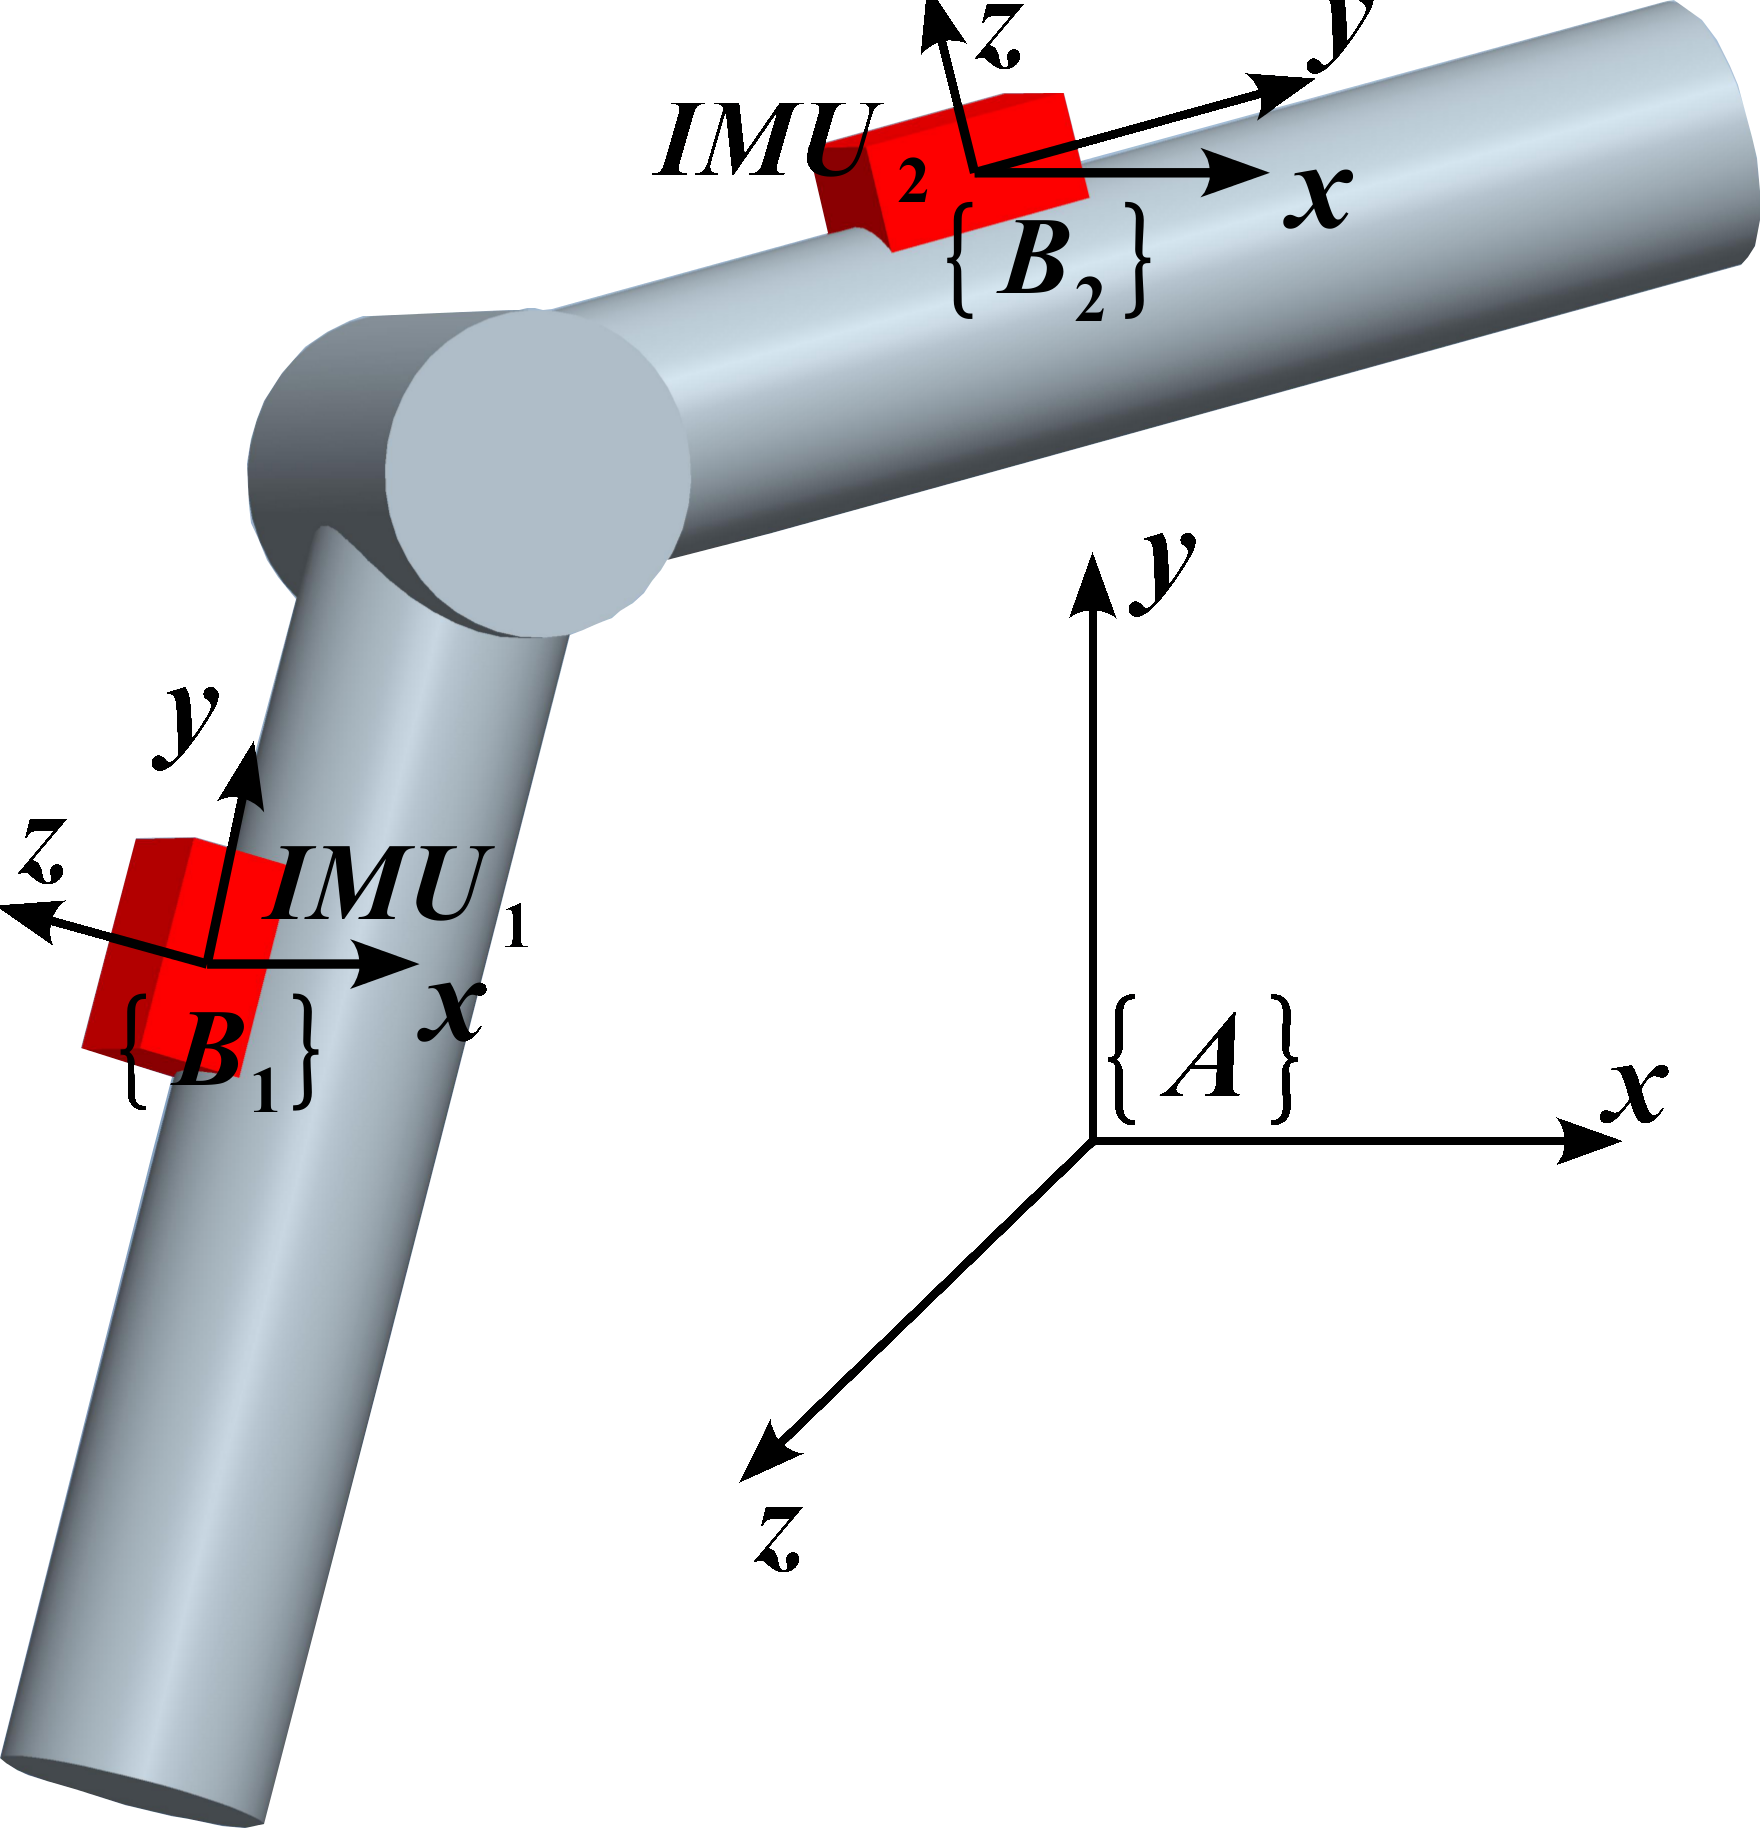
\includegraphics[scale=0.5]{TwoLinksOneJoint.png}
\caption{Simple structure with two link connected by a revolute joint}
\label{TwoLinksOneJoint}
\end{figure}

\subparagraph{Orientation between two IMU sensors}

The use of two IMUs in a kinematic chain as shown in Fig.~\ref{TwoLinksOneJoint} returns two orientations, namely $^{b{_1}}_a \hat{\overline{q}}$ and $^{b{_2}}_a \hat{\overline{q}}$ in the inertial frames $\{ B_1 \}$ and $\{ B_2 \}$ of body $1$ and $2$, respectively, with respect to a common frame $\{ A \}$. The relative orientation of the bodies can be readily obtained by
\begin{equation}
\label{eq4_18}
{^{b_1}_{b_2}\hat{\overline{q}}} = {_{a}^{b_2}\hat{\overline{q}}^{*}} \otimes {_{a}^{b_1}\hat{\overline{q}}}.
\end{equation}

However, it is also possible to apply the Madgwick filter to the measurements read from the two IMUs, to obtain ${^{b_1}_{b_2}\hat{\overline{q}}}$ directly, since it applies to the relative orientation of two bodies.

Thus, having the accelerometer, gyroscope and magnetometer measurements, $\overline{g}_{b_i}$, $^{b_i} \Omega$ and $\overline{m}_{b_i}$, in frame $\{ B_i \}$, for $i=1,2$ bodies, the terms of the correction factor shown in~\eqref{eq4_10} change correspondingly, that is, \eqref{eq4_10bis} becomes
\begin{equation}
\label{eq4_19}
^{b_1}_{b_2} \bar{q}_k = \frac{1}{2} {^{b_1}_{b_2} \bar{q}_{k-1}} \otimes {^{b_1}_{b_2} \Omega_k},  \quad k = 1,2,3 \dots n,
\end{equation}
where
\begin{equation}
\label{eq4_20}
{^{b_1}_{b_2} \Omega_k} = {^{b_2} \Omega_k} - {^{b_1}_{b_2} \bar{q}_{k-1}} \otimes {^{b_1} \Omega_k} \otimes {^{b_1}_{b_2} \bar{q}^{*}_{k-1}},
\end{equation}
is the angular rate of frame $\{ B_2 \}$ with respect the frame $\{ B_1 \}$. Then,~\eqref{eq4_16}), becomes
\begin{equation}
\begin{split}
\label{eq4_21}
\nabla f_{g,m}(^{b_1}_{b_2} \bar{q}_k,\bar{g}_{b_2},\bar{g}_{b_1},\bar{m}_{b_2},\bar{m}_{b_1}) = J_{g,m}^T(^{b_1}_{b_2} \bar{q}_k, \bar{g_{b_2}},\bar{m_{b_2}}) \\ {f}_{g,m}(^{b_1}_{b_2} \bar{q}_k,\bar{g}_{b_2},\bar{g}_{b_1},\bar{m}_{b_2},\bar{m}_{b_1}).
\end{split}
\end{equation}
Thus, the relative quaternion at step $(k+1)$, is given by
\begin{equation}
\label{eq4_22}
^{b_1}_{b_2} q_{k+1} = ^{b_1}_{b_2} \bar{q}_k - \beta \frac{\nabla f_{g,m}(^{b_1}_{b_2} \bar{q}_k,\bar{g}_{b_2},\bar{g}_{b_1},\bar{m}_{b_2},\bar{m}_{b_1}) }{\vert \vert \nabla f_{g,m}(^{b_1}_{b_2} \bar{q}_k,\bar{g}_{b_2},\bar{g}_{b_1},\bar{m}_{b_2},\bar{m}_{b_1})  \vert \vert}, \quad k = 0,1,2 \dots n.
\end{equation}

Algorithm~\ref{MadgwickAlgTwo} summarizes the steps followed to obtain the relative orientation of the two bodies.

\begin{algorithm}
\caption{Two IMUs Madgwick Discrete Filter at $n^{th}$ step}
\begin{algorithmic}[1]
\label{MadgwickAlgTwo}
\STATE Reading the current values of the accelerometers ($g_{{b_1}_n}$), magnetometers ($m_{{b_1}_n}$) and gyro rates ($\Omega_{{b_1}_n}$) in the local $IMU_1$ frame $\{B_1\}$
\STATE Normalizing gravity and magnetic field vector read from $IMU_1$ $\overline{g}_{{b_1}_n} = \frac{g_{{b_1}_n}}{\vert \vert g_{{b_1}_n} \vert \vert}$, $\overline{m}_{{b_1}_n} \frac{m_{{b_1}_n}}{\vert \vert m_{{b_1}_n} \vert \vert}$
\STATE Reading the current values of the accelerometers ($g_{{b_2}_n}$), magnetometers ($m_{{b_2}_n}$) and gyro rates ($\Omega_{{b_2}_n}$) in the local $IMU_2$ frame $\{B_2\}$
\STATE Normalizing gravity and magnetic field vector read from $IMU_2$ $\overline{g}_{{b_2}_n} = \frac{g_{{b_2}_n}}{\vert \vert g_{{b_2}_n} \vert \vert}$, $\overline{m}_{{b_2}_n} \frac{m_{{b_2}_n}}{\vert \vert m_{{b_2}_n} \vert \vert}$
\STATE Computing the objective function value $f_{g,m}({^{b_1}_{b_2}\hat{\overline{q}}_{n-1}},\overline{g}_{{b_2}_n},\overline{g}_{{b_1}_n},\overline{m}_{{b_2}_n},\overline{m}_{{b_1}_n})$ using equations (\ref{eq4_12}) and (\ref{eq4_14})
\STATE Computing the transpose of the Jacobian of the objective function $J^T_{g,m}(^{b_1}_{b_2}\hat{\overline{q}}_{n-1},\overline{g}_{{b_2}_n},\overline{m}_{{b_2}_n})$ using equations (\ref{eq4_13}) and (\ref{eq4_17})
\STATE Computing the correction terms $c_n =  \beta \frac{\nabla f}{\vert \vert \nabla f \vert \vert}$ using equation (\ref{eq4_16})
\STATE Computing the orientation quaternion time variation $^{b_1}_{b_2} \hat{q}_{d_n} =  (\frac{1}{2} {^{b_1}_{b_2}\hat{\overline{q}}_{n-1}} \otimes {^{b_1}_{b_2} \Omega_k}) - c_n$ using (\ref{eq4_20})
\STATE Computing the new orientation quaternion estimation given by its previouly one and its current time variation $^{b_1}_{b_2} \hat{q}_n = ^{b_1}_{b_2}\hat{\overline{q}}_{n-1} + ^{b_1}_{b_2} \hat{q}_{d_n} \Delta t$
\STATE Normalizing the new estimated quarternion $^{b_1}_{b_2} \hat{\overline{q}}_n = \frac{^{b_1}_{b_2} \hat{q}_n}{\vert \vert ^{b_1}_{b_2} \hat{q}_n \vert \vert}$
\end{algorithmic}
\end{algorithm}

\paragraph{(b) Hardware}

In this section, the IMU (Inertial Measurements Unit) sensors are described along with their interrogation and management by the filter. 
%The low-consumption, lightweight and potential for low-cost manufacture of these sensors opens up a wide range of solution. 
To reconstruct the hand posture 17 IMUs are rigidly attached to a glove that is worn by the hand. In particular, one device in mounted on each phalanx of each finger ($3x5=15$), one is mounted on the hand palm, and the last one is attached to the wrist of the glove. Fig.~\ref{fig:hardware} shows the complete hardware setup proposed as solution whose components are described below.
\begin{figure}[h]
\centering
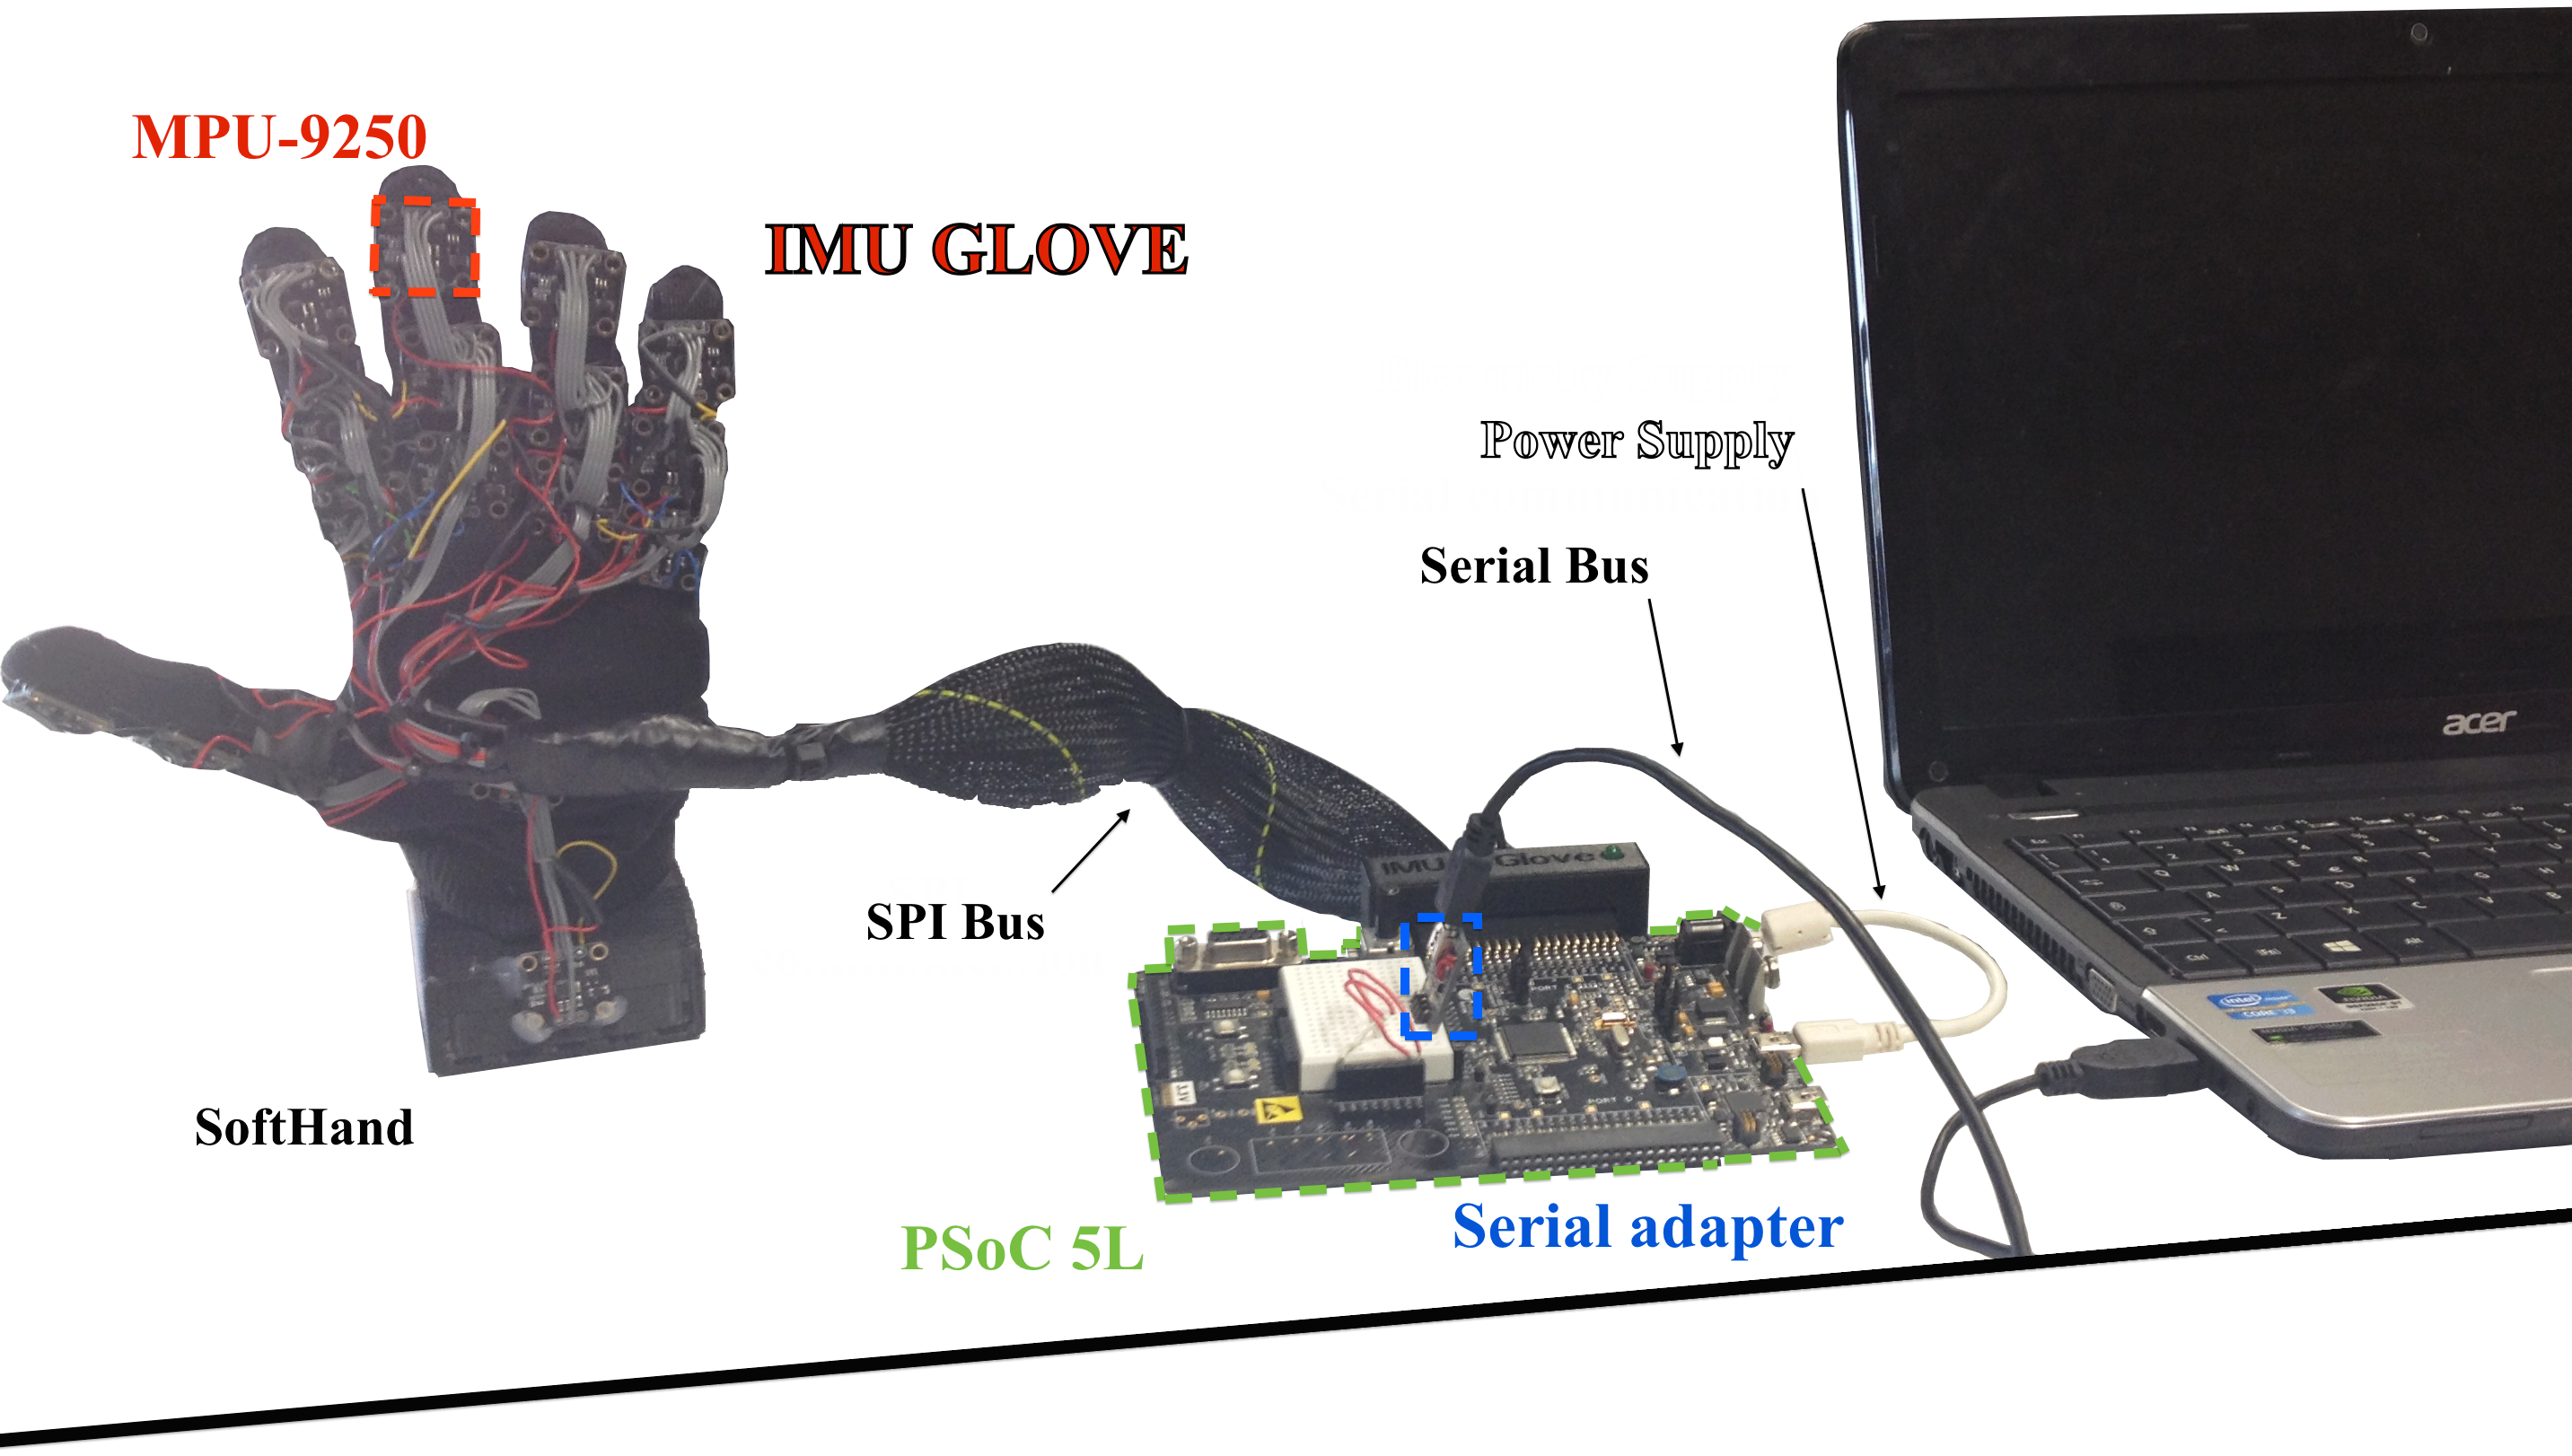
\includegraphics[scale=0.125]{hardware.png}
\caption{Complete hardware setup of the IMU-based glove for the Pisa/IIT SoftHand}
\label{fig:hardware}
\end{figure}



\subparagraph{MPU-9250}

Although the size of a generic IMU is very small, an accurate selection of the sensors to better assembly the glove led us to choose the device MPU-9250 by InvenSense~\cite{MPU9250}. 

\begin{figure}[h]
\centering
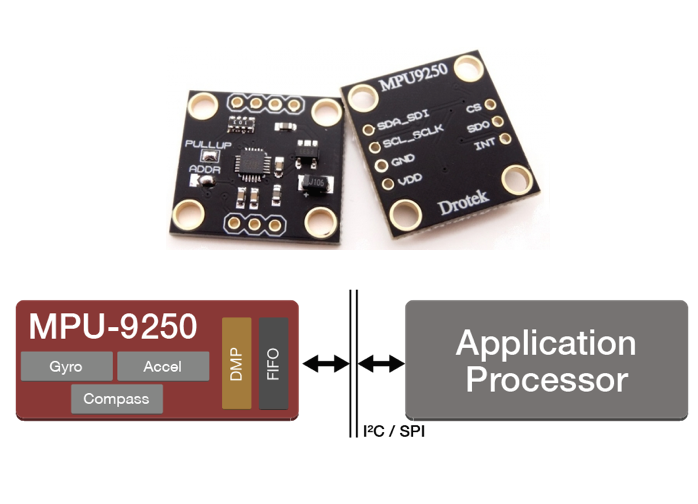
\includegraphics[scale=0.35]{mpu9250.png}
\caption{MPU-9250}
\label{fig:mpu9250}
\end{figure}

This is a System in Package device (SiP) that combines two chips: the MPU-6500 device (used in the first feasibility study \cite{Santaera:ICRA:2015}) containing a 3-axis gyroscope and a 3-axis accelerometer, and the AK8963, a market leading 3-axis digital compass. In particular:

\begin{itemize}
\item[$\cdot$] \textit{Accelerometer}: Use separate proof masses for each axis. Acceleration along a particular axis induces displacement on the corresponding proof mass, and capacitive sensors detect the displacement differentially. The 3-analog information is digitized using individual on-chip 16-bit Analog-to-Digital Converters (ADCs) to sample each axis;

 \item[$\cdot$] \textit{Gyroscope}: There are three indipendet vibratory rate gyroscopes, wich detect rotation about the X, Y and Z axes. When the gyroscope are rotated about any of sense axes, the Coriolis force causes a vibration that is detected by a capacitive pickoff. The resulting signal is amplified, demodulated and filtered to produce a voltage proportional to the angular rate. This voltage, as for the accelerometer, pass thorugh a ADC providing digital outputs.

 \item[$\cdot$] \textit{Magnetometer}: The 3-axis magnetometer uses higly sensitive Hall sensor technology. It detects a magnetic field in the X, Y and Z axes. As the other, each ADC has 16-bit resolution.
\end{itemize}

% \noindent The MPU-9250's technical features are summarized in the Table \ref{tab:mpu}.
% \begin{table}[tb]\footnotesize
% \caption{MPU-9250 features}
% \centering
% \label{tab:mpu}
% \begin{tabular}{l | c | l}
% \textbf{Part} & \textbf{Unit} &  \\ \hline \hline
% Gyro Full Scale Range & (deg/sec) &  $\begin{array}{l}   \pm 250 \\  \pm 500  \\ \pm 1000 \\ \pm \textbf{2000} \end{array}$  \\
% \rowcolor [gray]{.8}  \text{Gyro Rate Noise} &  (\text{dps}/$\sqrt{\text{Hz}}$)  & $\begin{array}{l}   0.01 \end{array}$  \\
% \text{Accel Full Scale Range} & (\text{g}) & $\begin{array}{l}   \pm 2 \\  \pm 4 \\  \pm \textbf{8} \\ \pm 16 \end{array}$ \\
% \rowcolor [gray]{.8} \text{Compass Full Scale Range} &($\mu\text{T}$) & $\begin{array}{l}   \pm \textbf{4800} \end{array} $\\
% \text{Digital Output} &  & $\begin{array}{l} \text{I}^2\text{C} \\ \textbf{SPI}   \end{array} $ \\
% \rowcolor [gray]{.8} \text{Logic Supply Voltage } & (\text{V}) & $\begin{array}{l} 1.7\text{V}\text{to}\text{VDD} \\ \textbf{VDD}   \end{array} $\\
% \text{Package Size} & (\text{mm}) & $\begin{array}{l} 3\text{x}3\text{x}1   \end{array}$
% \end{tabular}
% \end{table}


The output data from  axes sensors can be read from a 8-bit register. Each axis sensor presents two registers: the  up  and the low register. Thus, a complete information from a specific sensor occupies 48-bit. Considering, for example, the accelerometer there are 16-bit for the x axis, 16-bit for the y axis and 16-bit for the z axis.

Fig.~\ref{fig:axes} shows the orientation of the axes of sensitivity and the polarity of rotation.
\begin{figure}[h]
\centering
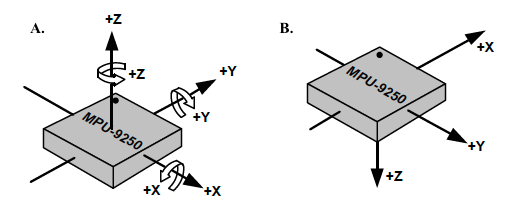
\includegraphics[scale=0.5]{axes_orientation.png}
\caption{A. Accelerometer and gyro orientation axes  B. Magnetometer orientation axes}
\label{fig:axes}
\end{figure}

As already mentioned, a complete sensorization of the glove and, therefore, of the hand needs 17 IMUs. This means that for keeping the time response of the system low, the communication between a master processing unit and each IMU becomes is crucial. The MPU-9250 supports two different types of digital communication: I$^2$C (Inter Integreted Circuit) and SPI (Serial Peripheral Interface). The I$^2$C maximum working frequency is 400Hz, while the SPI works at 1Mhz. Therefore, the SPI allows a faster communication and using the Slave-Select pin, it allows the user to use a single bus to overcome the problem of setting a unique address per sensor.

% In Figure~\ref{fig:spi}, the pin-out of a generic SPI communication is shown. In particular, the SPI is a 4-wire synchronous serial interface that uses two control lines and two data lines:
% \begin{itemize}
% \item[-] SCLK, clock - control line;
% \item[-] MOSI, master-output slave-input - data line;
% \item[-] MISO, master-input slave-output - data line;
% \item[-] SS,   slave select - control line.
% \end{itemize}

% \begin{figure}[h]
% \centering
% 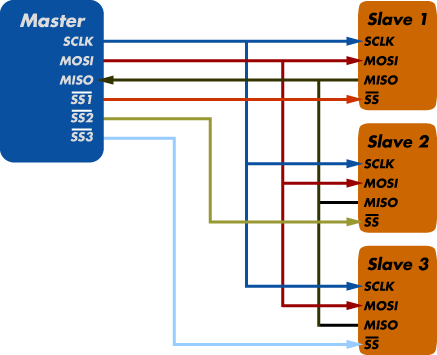
\includegraphics[scale=0.4]{spi.png}
% \caption{Scheme of SPI communication}
% \label{fig:spi}
% \end{figure}

In our work, the MPU-9250 always operates as a Slave device during standard Master-Slave SPI operation and to speed up communication between master and sensors, in our work three SPI bus are used~\ref{fig:IMU_Glove_bus}.
%In each bus the SCLK, the MISO and the MOSI pin are shared by all slaves devices, while each slave device requires its own SS line to communicate with the master. The SS pin goes low, (\textit{active}) when the transmission start, and comes back high (\textit{inactive}) at the end, so only one SS line is active at a time, ensuring that only one slave is selected at any given time.

\begin{figure}[h]
\centering
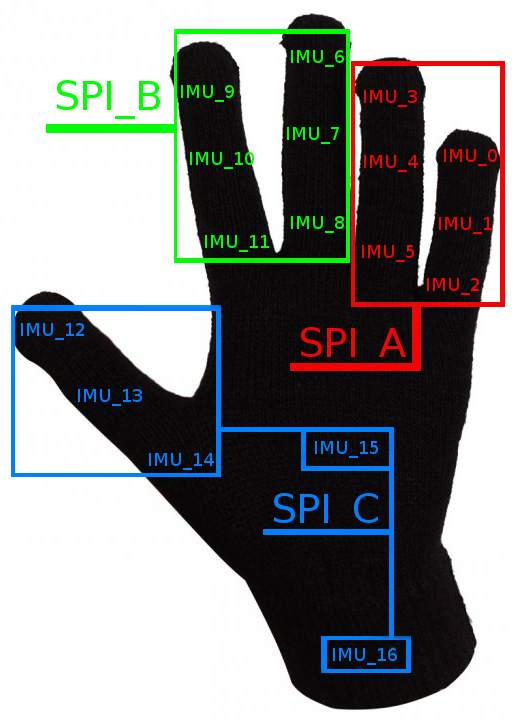
\includegraphics[scale=0.4]{Glove_IMU_SPI.png}
\caption{SPI bus used in the IMU Glove}
\label{fig:IMU_Glove_bus}
\end{figure}


\subparagraph{PSoC 5LP}

This is master. It is a micro-controller that support SPI communication with more than 17 pins to manage all slave devices. The microcontroller is be able to read the IMUs as well as to send data to the PC through a serial adapter, where the Magdwick Filter is implemented. The processing unit used is a PSoC mounted on the \textit{PSoC 5LP} board developed by Cypress Semiconductor \cite{PSOC5LP}. The PSoC is a low-power ARM \textsuperscript \textregistered Cortex - M3 based programmable system on chip devices offering unmatched high-precision analog and the flexibility to design custom system solutions. Combined with the free PSoC software development tools (PSoC Creator and
PSoC Programmer) from Cypress, this board is a good solution for applications who need different hardware devices and good time response. %in able to offer a large range of internal devices and solutions necessary to our application.

%more than sufficient for creating anything from basic microcontroller with embedded analog and digital functions to a highly complex system controller. Both the hardware system architecture and the software are supported by the PSoC
%software tools.
The PSoC integrated circuit is composed of a core, configurable analog and digital blocks, and programmable routing and interconnect. The configurable blocks in a PSoC are the biggest difference from other micro controllers. For this reason it can be associated to the FPGA microcontroller family (Field-Programmable Gate Array).
%\begin{figure}[h]
%\centering
%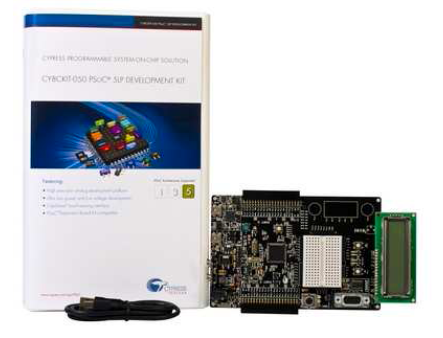
\includegraphics[scale=0.5]{psoc.png}
%\caption{PSoC 5LP}
%\label{fig:psoc}
%\end{figure}

%By using configurable analog and digital blocks, it is possible to create and change mixed-signal embedded applications. These blocks are designed by PSoC-Creator, an Integreted Design Environment (IDE).
%The development of the PSoC 5LP  and PSoC-Creator has permitted to managed  the IMUs easily.
%In our work the PSoC is used first to communicare with IMU then to send data read from sensors to computer.

%The first task of the microcontroller is to read data from the slave devices allowing a SPI communication. The SPI bus could be only one, but three separated buses were preferred to have greater control on the hardware system and to speed up the communication.
% \begin{figure}[h]
% \centering
% 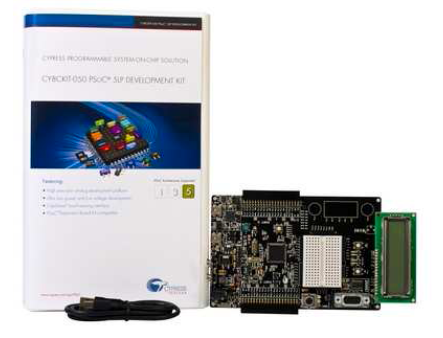
\includegraphics[scale=0.5]{psoc.png}
% \caption{SPI buses on the IMU glove}
% \label{fig:spibuses}
% \end{figure}
%After all IMU data are read, the data are stored in the EEPROM of the PSoC5 and are ready to be send to the PC. 
To communicate with the PC, the PSoC5 has a dual-channel USB. A first channel \textit{A} %of the highspeed USB interface is
is connected to the PSoC 5 in FIFO parallel mode to allow a fastest transfers between the USB host PC and the PSoC 5. A second channel \textit{B} is connected to the PSoC 5 in serial mode to allow a standard UART communication between the host PC and the PSoC5. However, channel A, commonly used to implement fast a communication, has a little communication buffer composed by 64 bytes, whereas to send all IMU data to the PC we would need more than 450 bytes. The channel B is a serial RS-232 channel and needs a Serial-USB converter to be connected to the PC. The PSoC 5LP mount on board presents an internal Serial-USB converter but its maximum baud rate is 115200, whereas we would need more than 900000.
Starting from these considerations, a different solution was implemented using on PSoC a standard serial communication and an external Serial-USB module to connected PSoC board to PC as described next.

\subparagraph{Serial Communication}

The communication between PSocC5 and PC was created exploiting the serial adapter 990 004~\cite{Serial_USB}. It is beneficial to connect a micro-controller and a logic circuit to a PC with a high data transfer rate. The heart of the module is the chip FT232R distributed by FTDI~\cite{FDTI_homepage}, which works with a supply tension of 3.3V, thus it possible to connect the device to another TTL peripheral o micro-controller in the range of 3.3V-5V without the problem to convert the signal RS232 to the TTL. The circuit fits in a $25 \times 18$mm square. The device is USB 2.0 compatible and it allows full speed at 1Mb/s.
% \begin{figure}[h]
% \centering
% 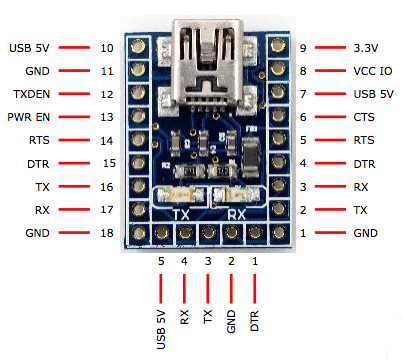
\includegraphics[scale=0.3]{usb_serial.png}
% \caption{Serial adapter}
% \label{fig:serial_adapter}
% \end{figure}


\paragraph{(c) Software}

To reconstruct the hand posture using the IMU glove two pieces of software are written. The first one is written in C and runs in the PSoC. This is called the firmware and it manages the IMU measurements as well as communication with the PC.
The second one is written in C++ and runs in the PC. This is called the application and it manages communication with the firmware and applies the Madgwick filter to measurments.
%The hardware described was managed in two fundamental step.  From one side there was the necessity to read IMU data and send its to computer, from the other side the sensor informations must be used to implement the algorithm for the  hand posture reconstruction.
%This was possible exploiting the PSoC5L where the \textit{Firmware} was installed and the \textit{Software} written in C++ in a Personal-Computer.

\subparagraph{Firmware on PSoC}

The firmware is written using the PSoC creator IDE developed by Cypress. This one offers an intuitive GUI to
%First of all the SPI communication was created between PSoC5L and the IMUs via software, where the PSoC5L  was the master and the IMUs the salves.  This was possible exploiting PSoC Creator, the software developed by Cypress. It
manage the internal PSoC devices represented as code blocks, to configure the PSoC input/output, and to write the code necessary to connect and work PSoC internal device and pin. % so all necessary pins of the PSoC's board were configured take advantage of the GUI offers by the IDE.
%Fig.~\ref{fig:firmwarepage1} shows how the three SPI bus are configurated and the relative pin used.%How the SPI communication was implemented is possible to view in the figure

% \begin{figure}[h]
% \centering
% 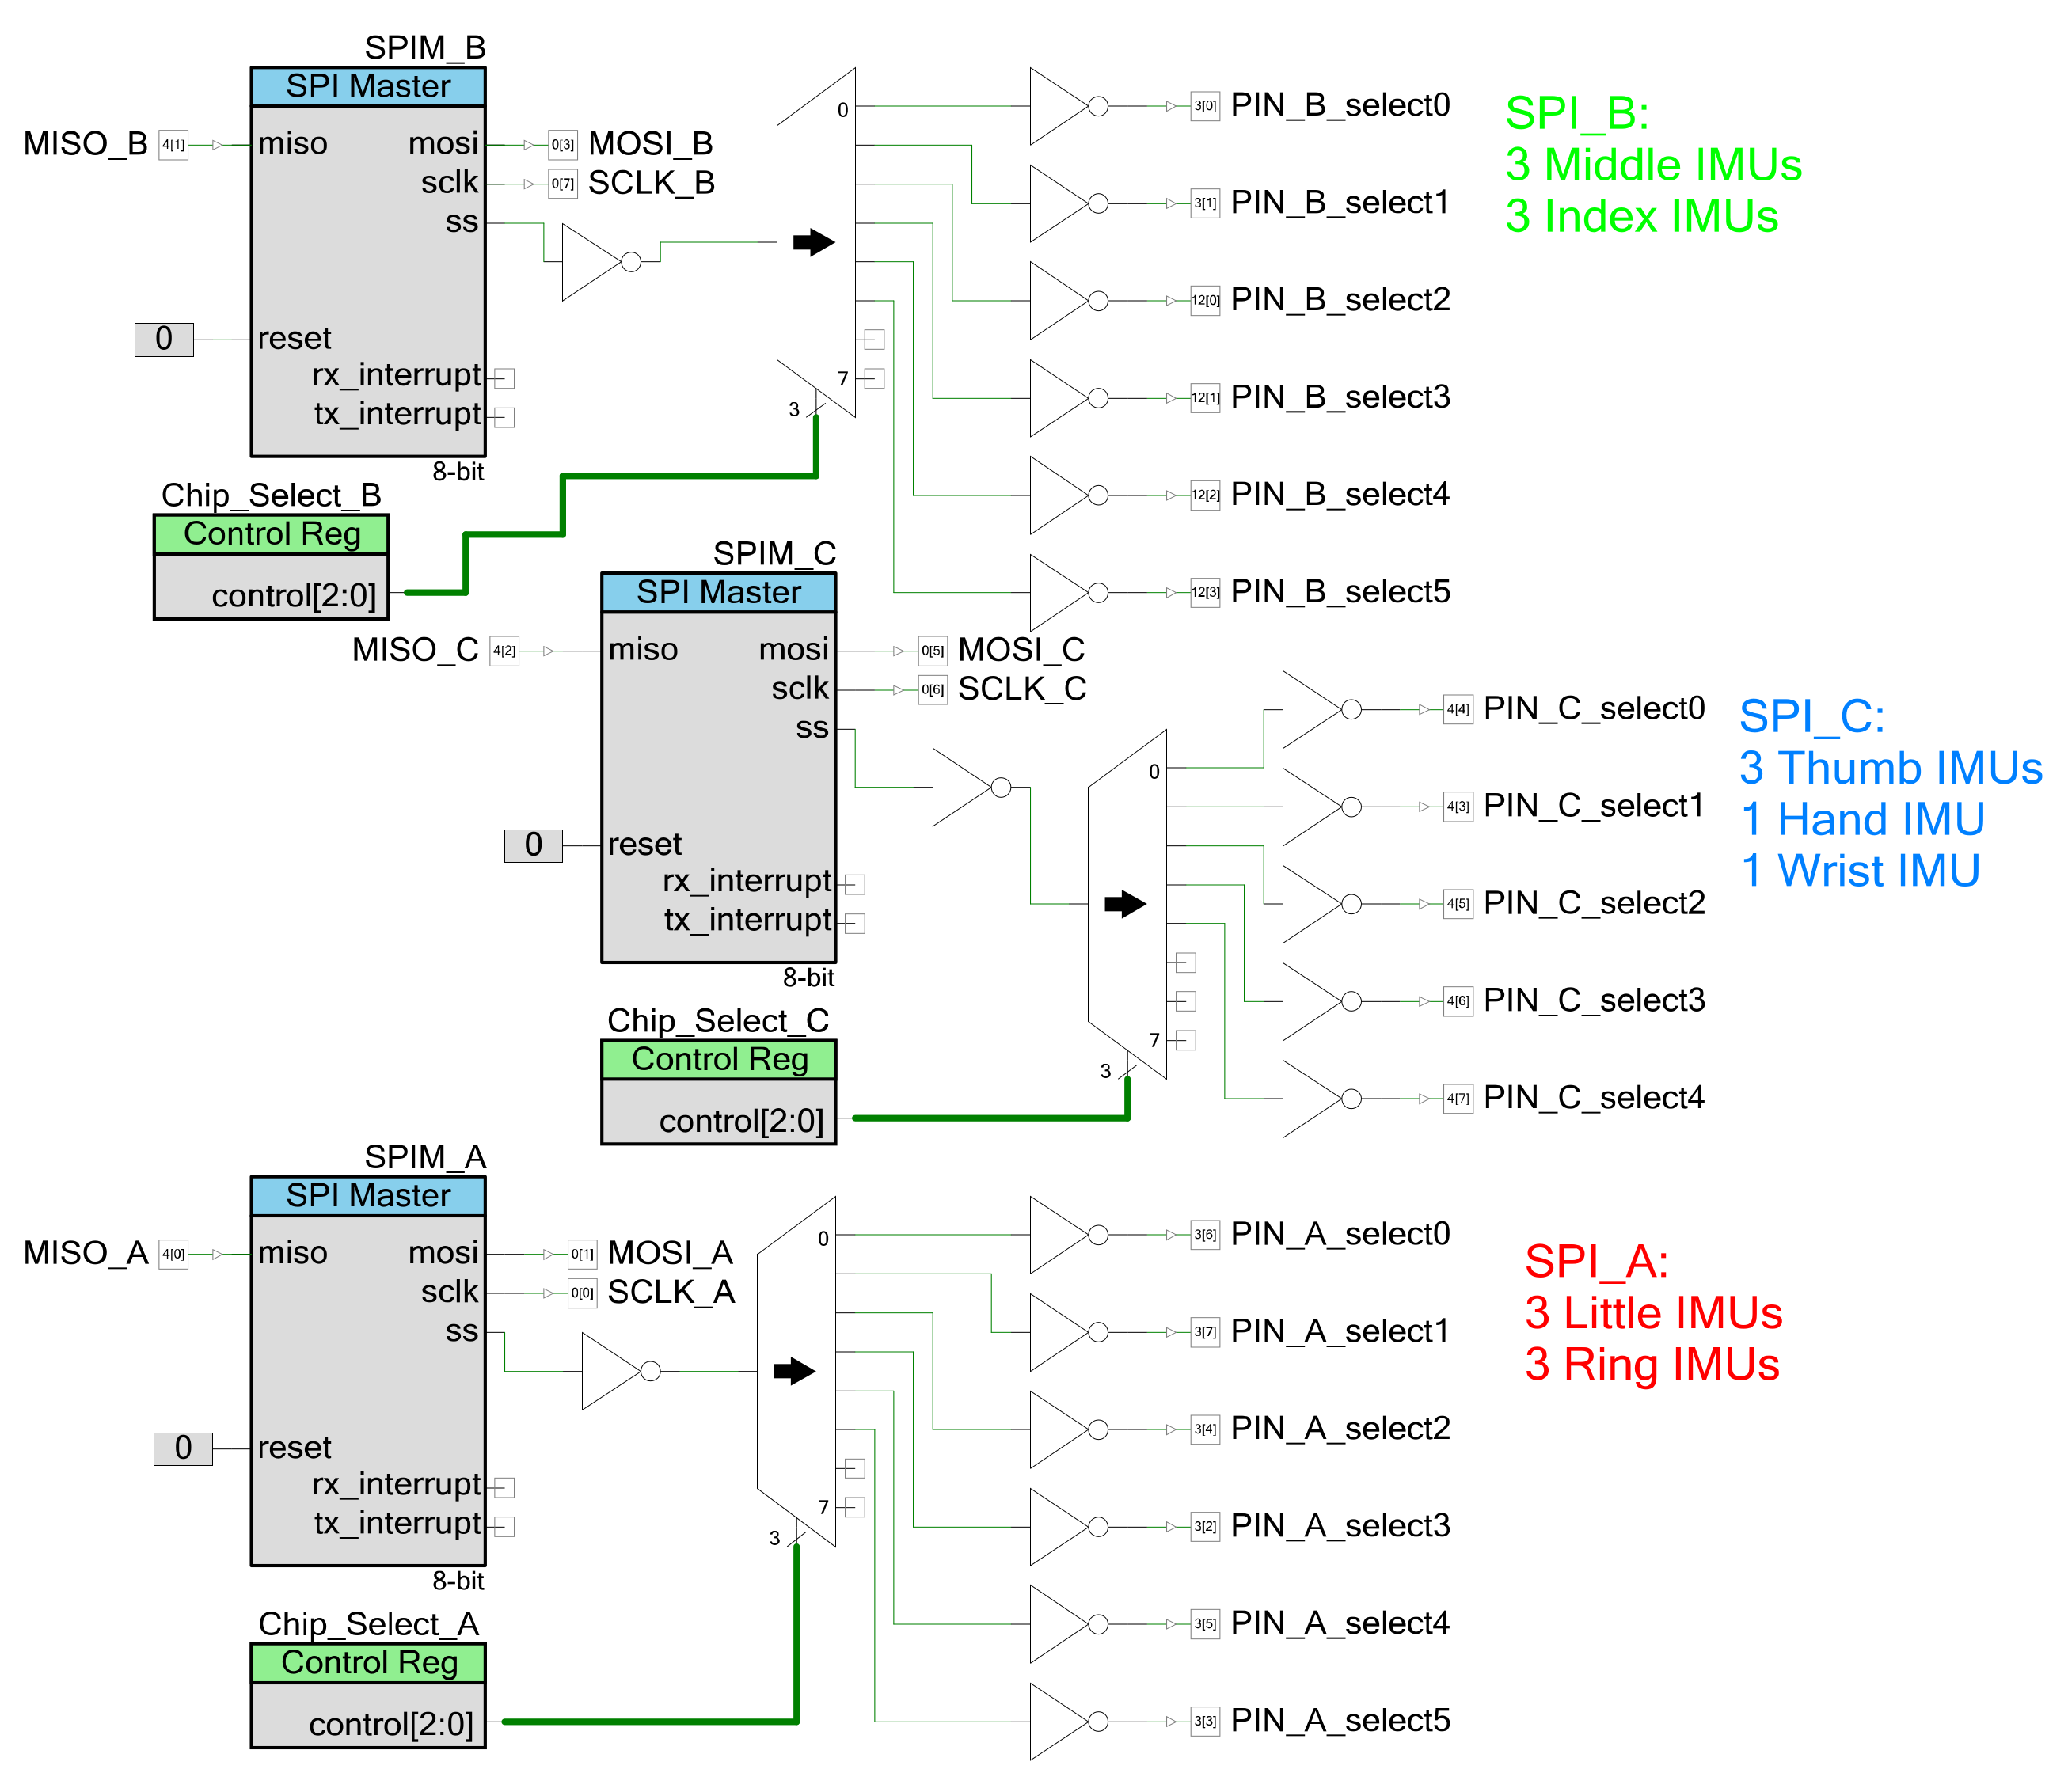
\includegraphics[scale=0.7]{Fimware_Page1.png}
% \caption{SPI blocks in the IDE}
% \label{fig:firmwarepage1}
% \end{figure}
Fig.~\ref{fig:psocfirmware} shows how the firmware manages the IMUs. %Guaranteed the communication between the sensor and the PSoc5L,  the firmware was written in the memory of the board, figure \ref{fig:psocfirmware}.
\begin{figure}[h]
\centering
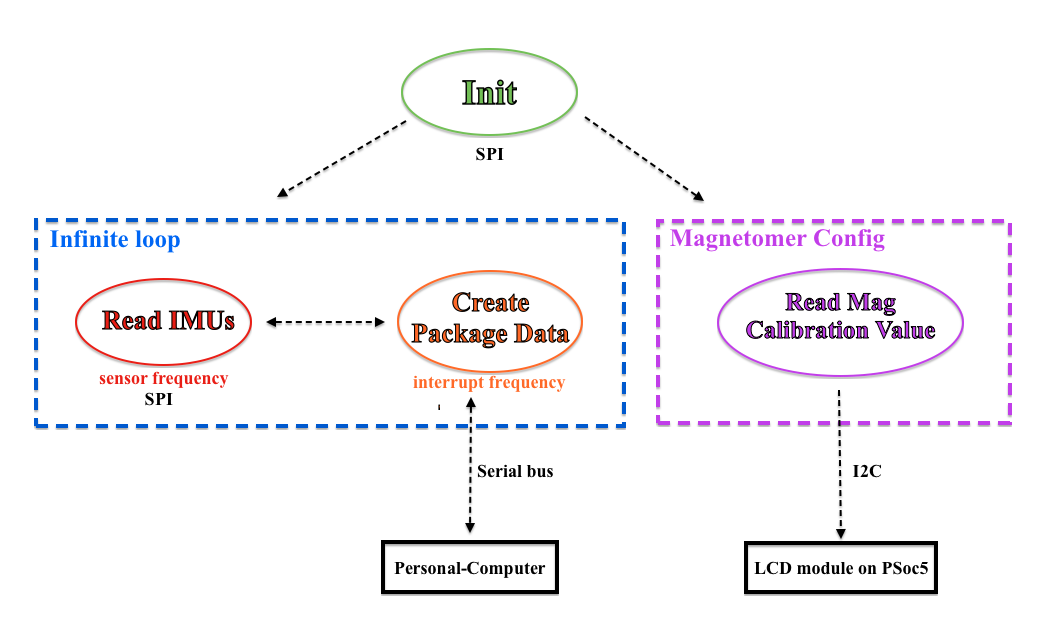
\includegraphics[scale=0.35]{firmware.png}
\caption{Scheme of the firmware written in the PSoC5L}
\label{fig:psocfirmware}
\end{figure}
In particular, there is an initalization phase \textit{Init}, where all IMU internal registers are set. This means configure, e.g. internal clock, type of communication, accelerometer, gyro full scale range, and so on.
After the initialization, the firmware can run in two different ways. The \textit{Magnetometer Config}, performed whenever there are new IMUs, helps to know sensitivity adjustment data for each magnetometer axis. In fact, due to constructive inaccuracies during the magnetometer installation on the MEMS, the magnetometer axis pose or orientation can be different between two IMUs. Therefore, the manufacturer stores in each IMU 8-bit register, three numbers (one for each axis), to equalize magnetic measurements between two o more IMU. In particular, these registers are:

\begin{enumerate}
\item[$\cdot$] $ASA_x[7:0]$: Magnetic sensor X-axis sensitivity adjustment value
\item[$\cdot$] $ASA_y[7:0]$: Magnetic sensor Y-axis sensitivity adjustment value
\item[$\cdot$] $ASA_z[7:0]$: Magnetic sensor Z-axis sensitivity adjustment value
\end{enumerate}

The sensitivity correction factor $s_a$ is given by %adjustment is done by the equation below
\begin{equation}
s_a  = \frac{ 0.5(ASA_a - 128)}{128} + 1,
\end{equation}
and for example the exact magnetic field on the $x$-axes is given by
\begin{equation}
H_{{adj}_x} = H_x s_x,
\end{equation}
where $H_x$ is the current data read from the measurement register, $ASA_x$ is the sensitivity $x$-axes correction factor and $H_{{adj}_x}$ is the real measurement.
%To Each values is possible to view on the LCD module on the PsoC's board via I2C.
All magnetometer correction factors are computed, and then they are store on the PC hard disk to correct the current data read from PSoC. %The magnetometer config step runs only one time, because  the adjustment parameters, once known, are stored by the user in the C++ code in the Personal-Computer.

After the initialization phase, the firmware will run in an \textit{Infinite loop} phase. This is subdivided in two independent sections
\begin{enumerate}
\item[$\cdot$] \textit{Read IMUs}: An internal counter each $20$ms (50Hz) generates an interrupt where IMUs are sequentially read and the output data stored in 3 different matrices
                          \begin{enumerate}
                          \item[-] Acc $\in \Re ^{17 \text{x} 3}$
                          \item[-] Gyro $\in \Re ^{17 \text{x} 3}$
                          \item[-] Mag $\in \Re ^{17 \text{x} 3}$
                          \end{enumerate}
                          The maximum frequency is the lowest one among the three sensors, and in particular the magnetometer has the lowest refresh frequency 100Hz.
\item[$\cdot$] \textit{Create Package Data}:  Between two subsequent interrupt, the matrices are reorganized in a package following the communication protocol depicted in Fig.~\ref{fig:package} with a total length of 462 bytes.

\begin{figure}[h]
\centering
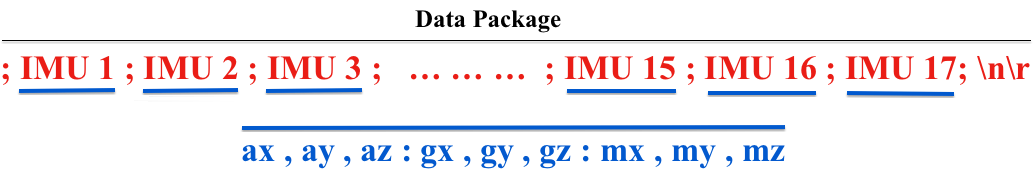
\includegraphics[scale=0.3]{datapackage.png}
\caption{Data package sent to  the PC}
\label{fig:package}
\end{figure}

% \noindent where its length is
% \begin{equation*}
% \displaystyle  \left. \begin{array}{lccc}
% \text{int} & \text{ax},\quad \cdots, \quad \text{mz}  & = & 2 \text{byte} \\
% \text{char} & , & = & 1 \text{byte} \\
% \text{char} & : & = & 1 \text{byte} \\
% \text{char} & ; & = & 1 \text{byte} \\
% \text{char} & \backslash \text{r} & = & 1 \text{byte} \\
% \text{char} & \backslash \text{n} & = & 1 \text{byte}
% \end{array} \right\rbrace \;
% \begin{array}{lcl}
% \textcolor{blue}{\text{int}} \; = \; 9 \; \cdot \; 17 \; & = & 306 \; \text{byte} \\
% \textcolor{blue}{\text{char}} \; = \; 8  \; \cdot \;+\; \; \textcolor{red}{\text{char}} \; \cdot \; 20  & = & 156 \; \text{byte}  \\
% & & \\ \hline
%  & & \text{462 byte}
% \end{array}
% \end{equation*}

The interrupt selecting the IMU reading and the data sending routines is generated using a PWM block. Similarly, the communication with the PC is implemented using an UART block.%, as shown in Figure~\ref{fig:firmwarepage1}

%The sent of this package is regulated by an interrupt every 50Hz via Serial bus.  The serial bus is managed developing PSoC Creator too. The frequency of interrupt is created by PWM block while for the serial communication a UART block is implemented, figure \ref{fig:firmwarepage1}.

% \begin{figure}[h]
% \centering
% 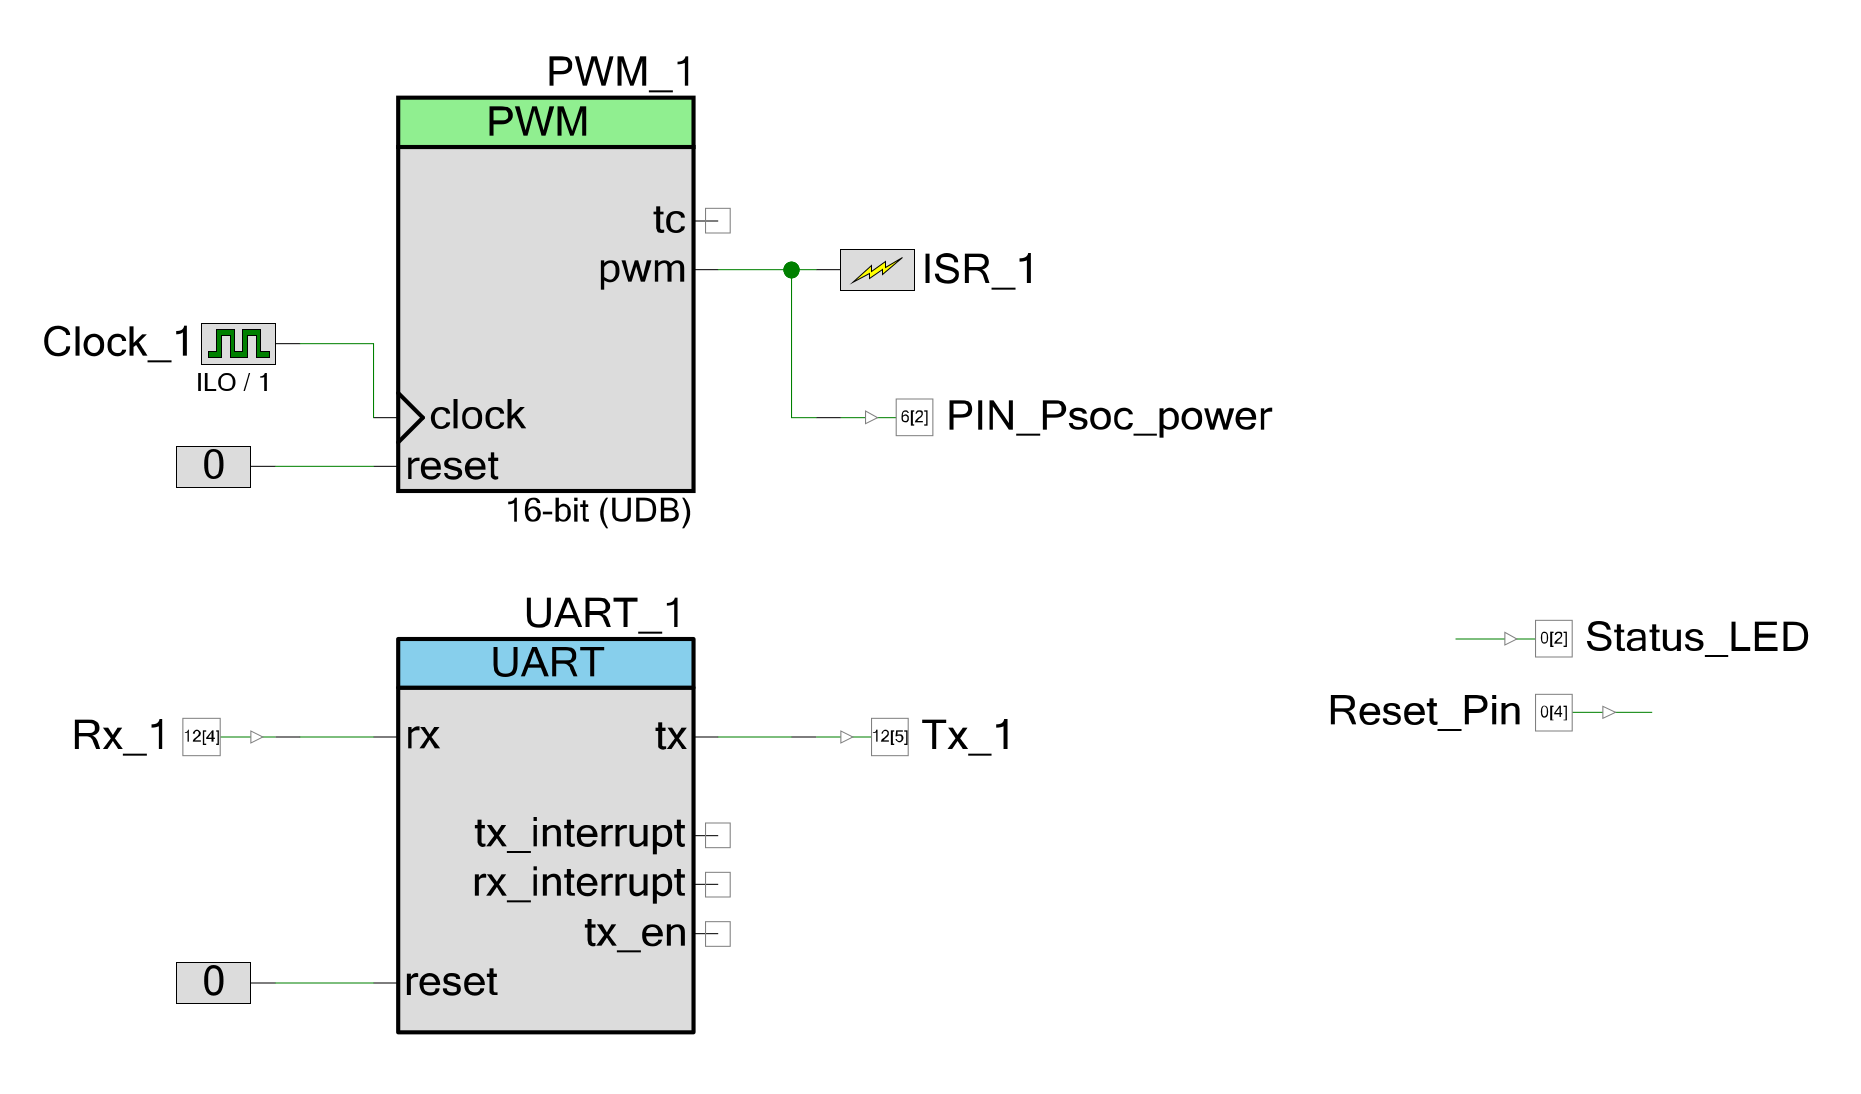
\includegraphics[scale=0.8]{Fimware_Page2.png}
% \caption{Interrupt and UART blocks in the IDE}
% \label{fig:firmwarepage1}
% \end{figure}

\end{enumerate}

\subparagraph{C++ code on PC}
%The code on PC implements, from data read by PSoC, the Madgwick algorithm between two IMUs. A scheme of the code is shown in 


\begin{figure}[h]
\centering
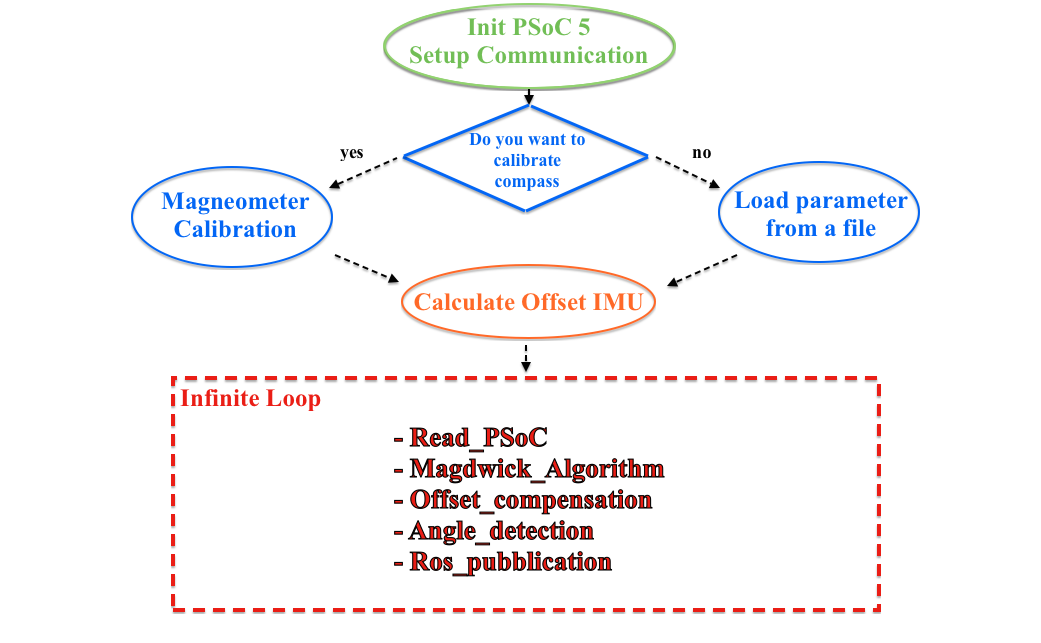
\includegraphics[scale=0.35]{code_c.png}
\caption{Code C++ implemented in the PC}
\label{fig:code_c}
\end{figure}

During an initial phase, the communication with the PSoC is configured. Then, the user decides whether to change or not the magnetometer calibration factors. 
%If the user decides to change the magnetometer calibration factors, a special function will run, and the new compass correction parameter will be stored in a file.txt to be load in the future. Magnetometer calibration takes about 50-60 seconds to compute all magnetometer correction factors.
If the user decides to keep the previous magnetometer corrector factors, the application applies the Madgwick filter to the IMU measurements to compute the offset angles between IMUs due to mounting inaccuracies. After these initial stages, the application enters in an infinite loop where it computes the relative orientation and the joint angles values from the current IMU measurements. Fig.~\ref{fig:code_c} summarizes the tasks and phases performed by the application.

%Once the offset quaternion is detected, the infinite loop starts calculating the desired joint angles.

\paragraph{(d) Validation}

In order to validate the hand posture reconstructed using the IMU glove, to demonstrate the potential of the proposed solution and its application for Task 3.3, some simple experiments have been performed on object recognition based on the hand configuration after grasping the object.

To validate the hand posture, a Pisa/IIT SoftHand is dressed with the IMU glove. Online visualization of the hand posture is programmed wth ROS (Robot Operating System) \cite{Ros_homepage}. Fig.~\ref{fig:hand_reconstruction_1} shows three different examples of hand posture reconstruction. A video was shot during a \href{https://www.youtube.com/watch?v=0oVha0Q1vWM}{static} and a \href{https://www.youtube.com/watch?v=bceOXa990-Q}{dynamic} configuration that validate the solution qualitatively.

\begin{figure}[h]
\centering
\mbox{
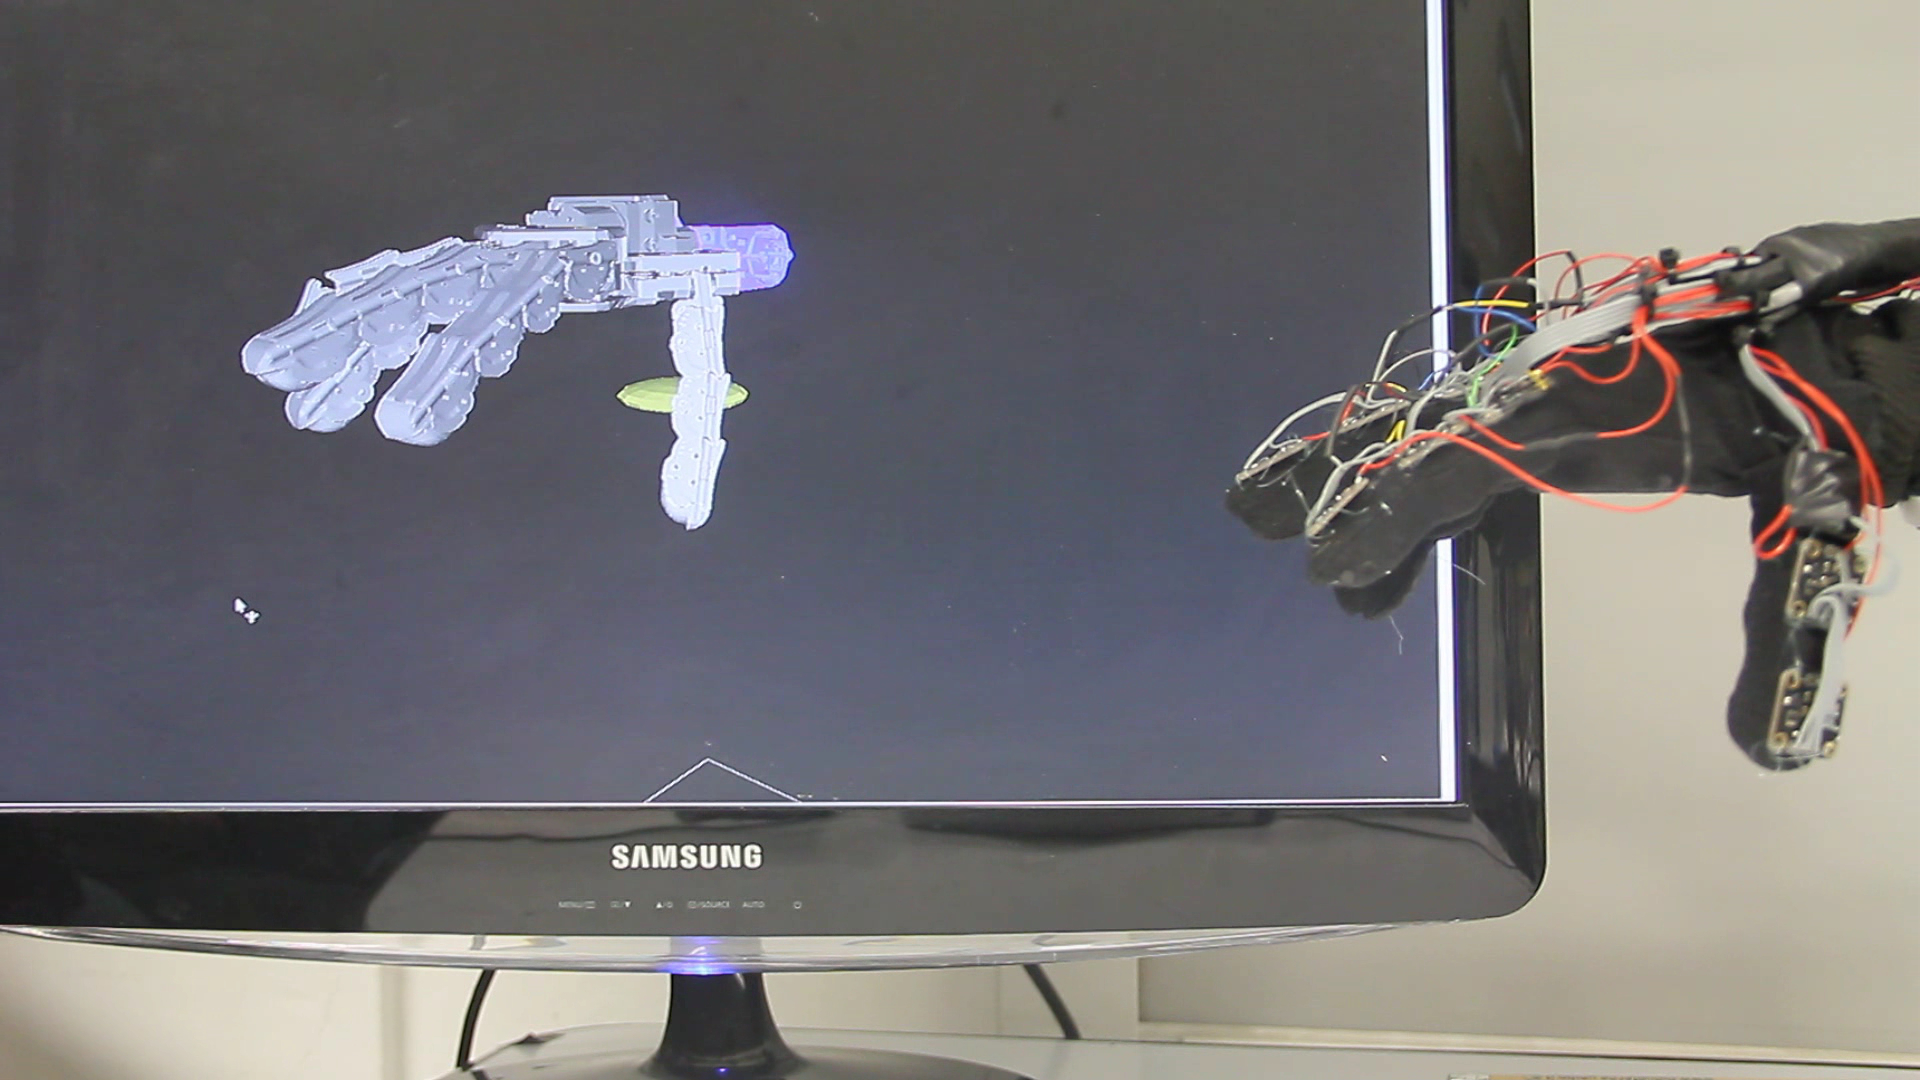
\includegraphics[width=0.33\linewidth]{Hand_Movement_1.png}
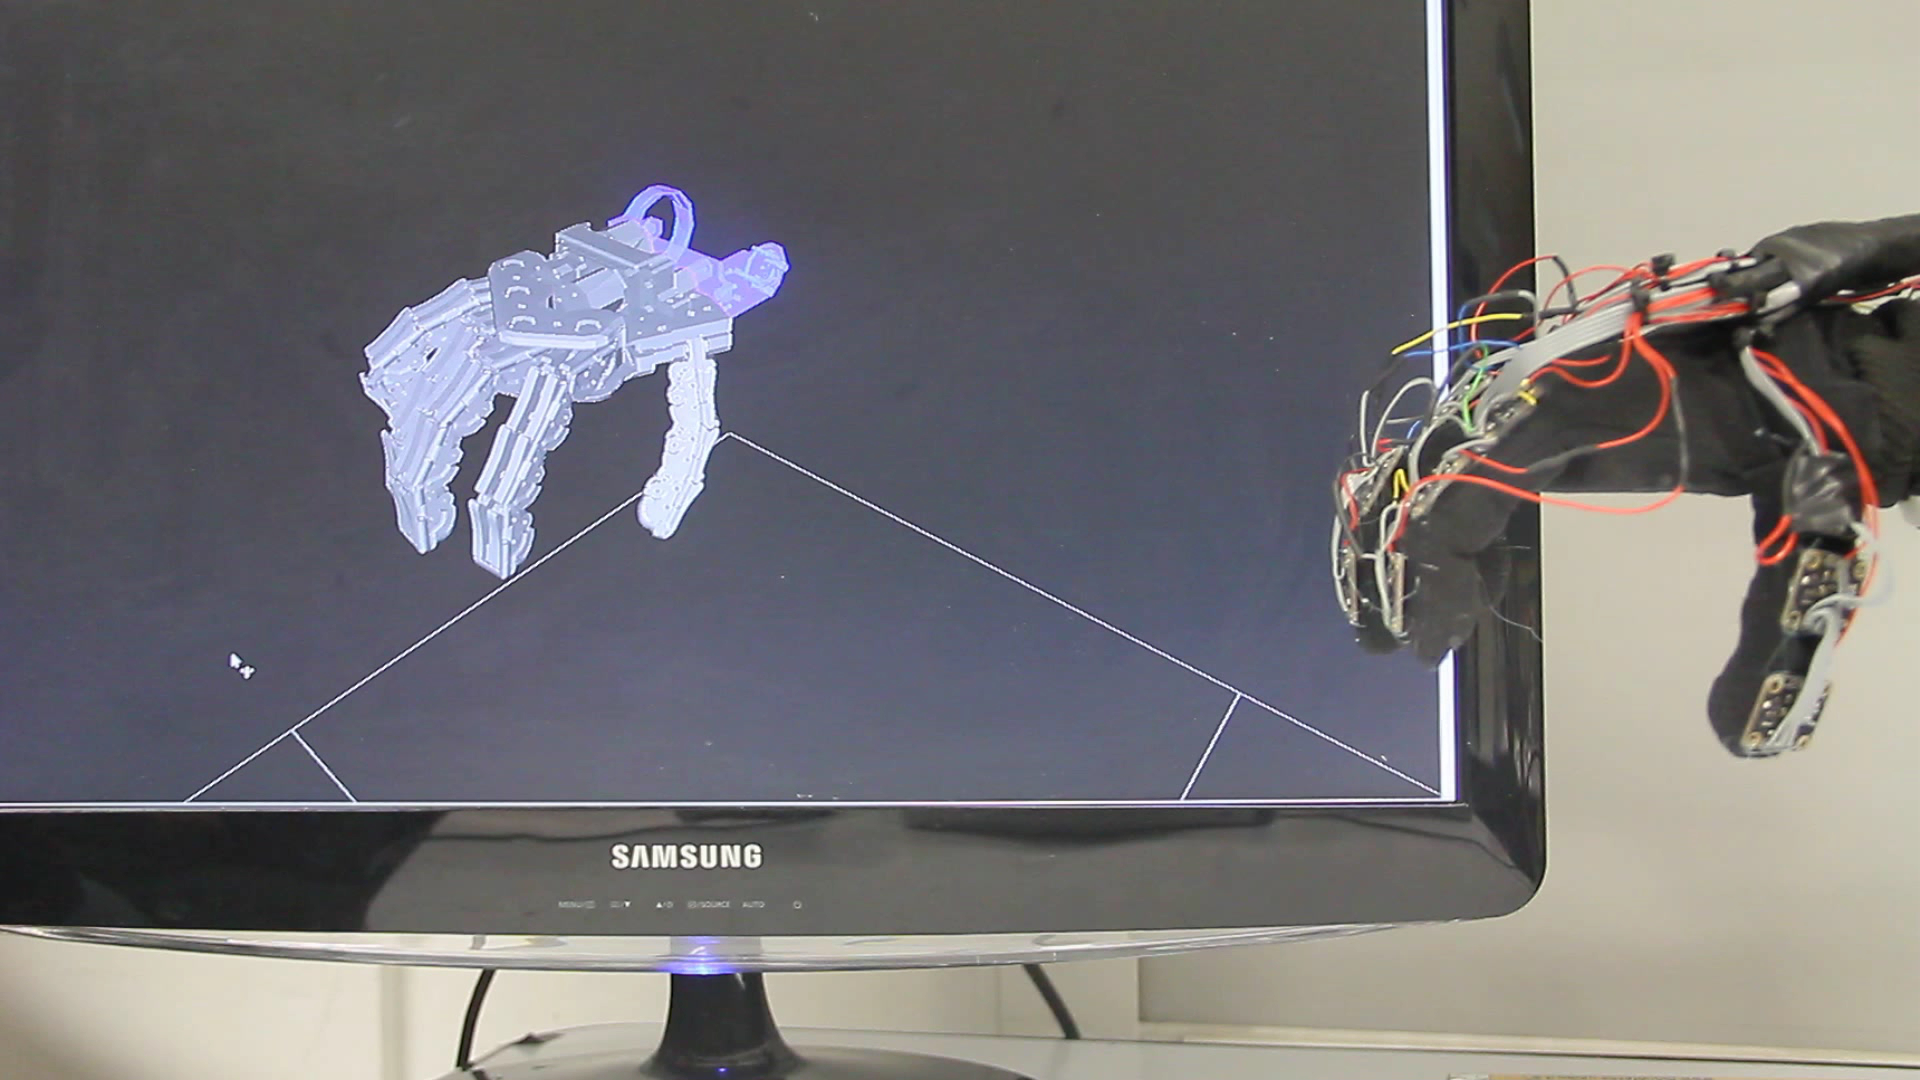
\includegraphics[width=0.33\linewidth]{Hand_Movement_2.png}
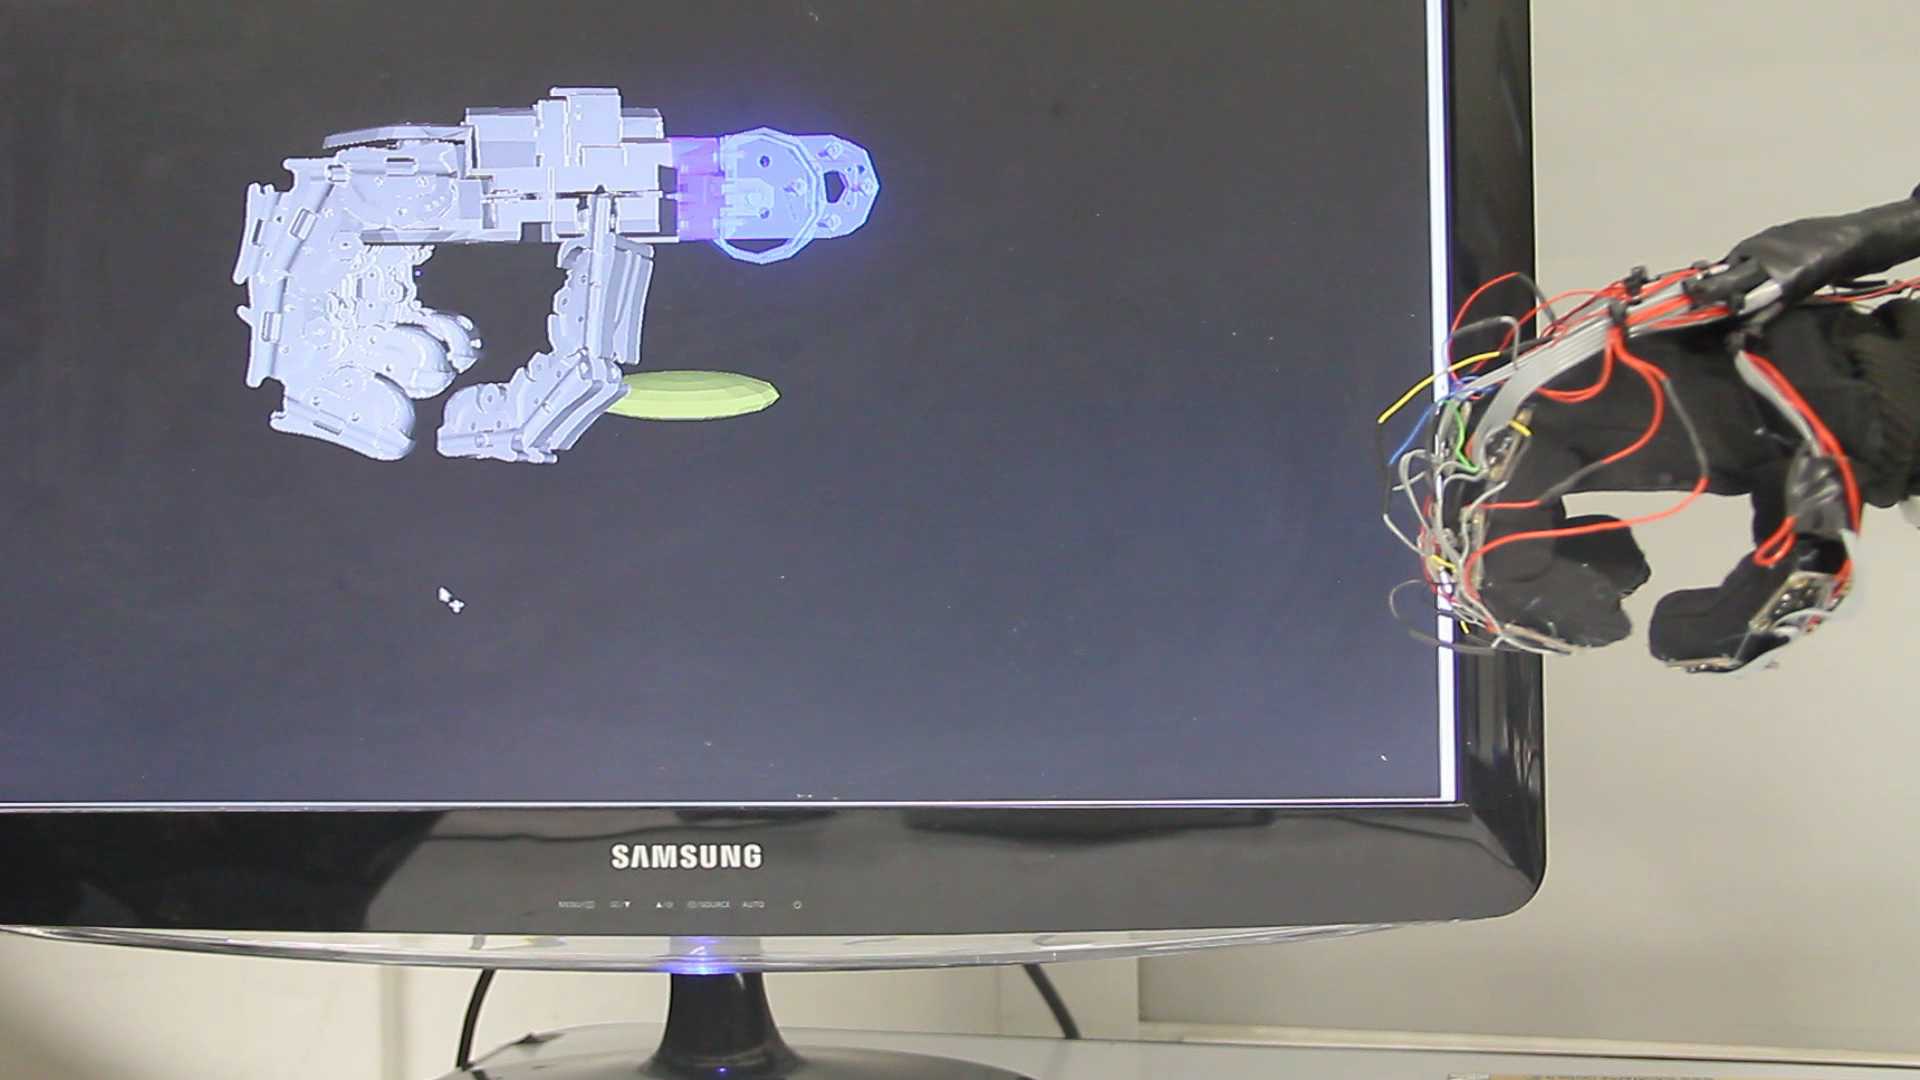
\includegraphics[width=0.33\linewidth]{Hand_Movement_3.png}
}
\caption{Hand posture reconstruction examples}
\label{fig:hand_reconstruction_1}
\end{figure}


Next, we challenge the proposed solution to recognized a grasped object based on the resulting hand configuration and using a naive approach. To this end, a set of five cups are used, where actually four belong to the PaCMan object database~\cite{PACMAN_datasets}. The cup sizes are presented in Table~\ref{tab:cups}, and it is worth nothing that, due their similarity, vision-based recognition techniques may present difficulties due to scaling issues.

\begin{table}[b]\footnotesize
\begin{tabular}{cc} \hline \hline
Cups Number & Diamter \\ \hline
\#1 & 55mm \\
\#2 & 76mm \\
\#3 & 82mm \\
\#4 & 90mm \\
\#5 & 98mm.
\end{tabular}
\caption{Probed Cups}
\label{tab:cups}
\end{table}

The object recognition experiments is composed by two different steps: \textit{Learn} and \textit{Recognize}.
The hand movements (open/close) are managed by a simple PID controller. The $K_p$, $K_d$ and $K_i$ parameters of the PID controller are set such that the hand squeezing force is low. In these conditions, the hand is not able to grasp an object, but behaves as a probe.

In the learning phase, the hand probes an object and the software running on the PC writes 20 row elements in a database. The row is composed by 1 number that identifies the object and 19 numbers that report the corresponding joint angles values (4 for little, 4 for ring, 4 for middle, 4 index and 3 for thumb).

In the recognition phase, the software reads the database and create in memory a matrix $O_{bj} \in \mathbb{R}^{n \times 20}$, where $n$ is the number of learned objects. when the hand closes and probes the current object, the software compares the current joint angles values with the values recorded during the learning phase. The match uses a brute force root mean square error minimizer. Here, the software returns $n$ different numbers $m_n$ representing the distance of each of the $n$ hand recorded poses to the current hand pose. The object in database whose hand pose signature is closest to the current one, has the smallest $m_n$ number. Explicitly, the distance $m_n$ is given by
\begin{equation}
m_n = \sqrt{(C_{angle_{1}} - O_{n_{angle_{1}}})^2 + \cdots + (C_{angle_{19}} - O_{n_{angle_{19}}})^2 },
\end{equation}
where $C_{angle_{k}}$ is the $k^{th}$ hand current joint angles value, $O_{n_{angle_{k}}}$ is the $k^{th}$ joint angles value corresponding to the $i^{th}$ object, for $k=1, 2 , \cdots , 19$ joints and $i=1,2, \cdots, n$ objects.

%With a large number of learned object ($n$) this object recognition strategy could require a large time to match current joints angles values with values recorded in the object database. In future work, we will investigate more efficient strategies (with respect to the current brute force search) to quickly match the current joint angles values with the recorded ones, and to being able to increase object database data types considering, for example, also grasping forces as features.

Even with this naive recognizer, the proposed solution was successful in discriminating the cups as shown in Fig. \ref{fig:Object_1}. For more in-sight on the recognition examples, we suggest to see videos by clicking on \href{https://www.youtube.com/watch?v=d_WPQ3WmHRg}{Object 1}, \href{https://www.youtube.com/watch?v=PG38VObdl6o}{Object 2}, \href{https://www.youtube.com/watch?v=bIYhLXm90hc}{Object $3_a$}, \href{https://www.youtube.com/watch?v=IXVlBAoGKho}{Object $3_b$}, \href{https://www.youtube.com/watch?v=Efmm6-JHcxU}{Object $4_a$}, \href{https://www.youtube.com/watch?v=NZElSV_AnJ4}{Object $4_b$}, \href{https://www.youtube.com/watch?v=mDDb5oTaHzM}{Object $5_a$} and \href{https://www.youtube.com/watch?v=sLzU39zffFY}{Object $5_b$}, where the subscripts $_a$ or $_b$ denote if the hand probes the cup handle or no, in this case the cup is recorded as two different objects.

\begin{figure}[h]
\centering
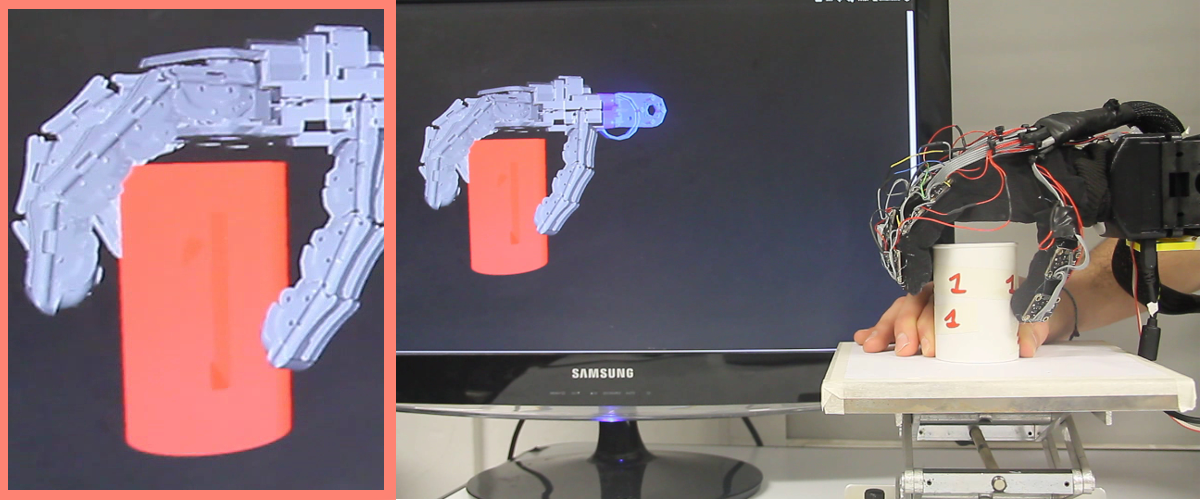
\includegraphics[width=0.9\linewidth]{Object_1.png}
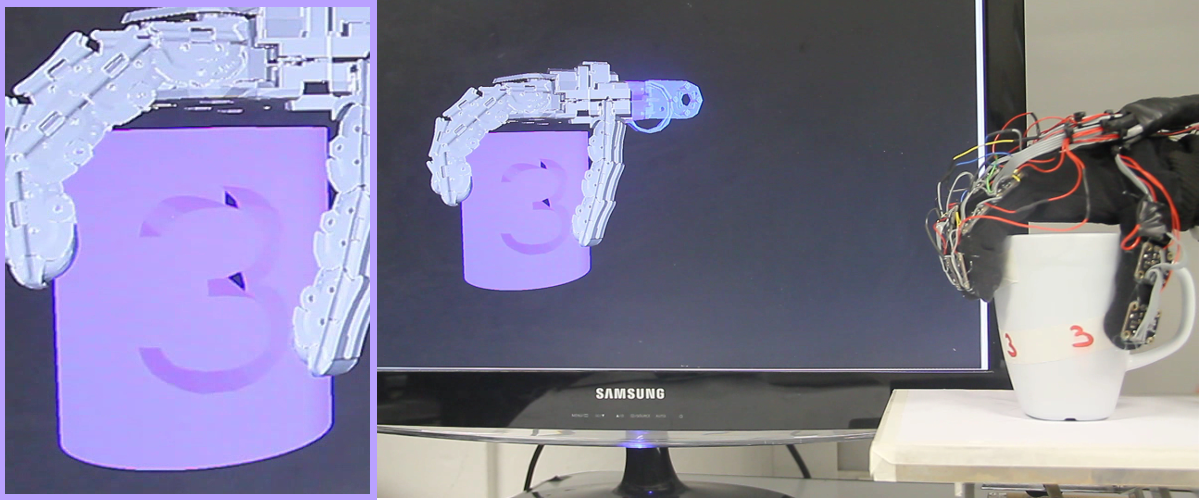
\includegraphics[width=0.9\linewidth]{Object_3.png}
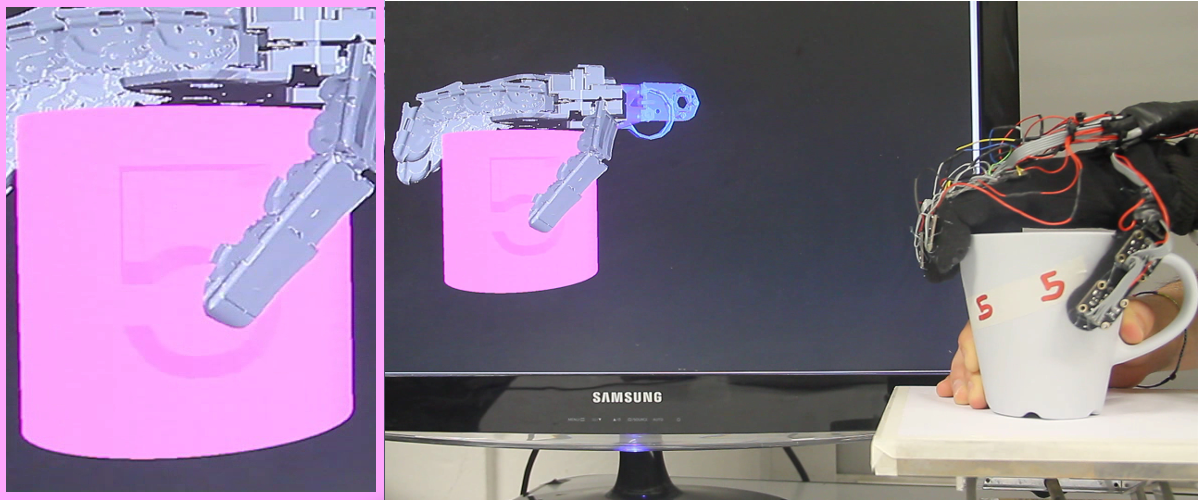
\includegraphics[width=0.9\linewidth]{Object_5.png}
\caption{Object recognition examples using the same cup of different sizes.}
\label{fig:Object_1}
\end{figure}